Přehled současného stavu se věnuje základnímu anatomickému popisu srdce společně
s úvodem do jeho fyziologie a elektrofyziologie ve spojení s neurofyziologickými
vlivy. Dále jsou zde popsány principy vyšetřovacích metod v kardiologii,
konkrétně oblast měření, zpracování a analýza elektrického záznamu srdeční
aktivity. Závěr kapitoly je věnován detailnějšímu rozboru variability srdeční
frekvence (HRV), která je předmětem analýzy zpracovaného EKG záznamu v rámci
této práce.

\subsection{Srdce}
\label{section:heart}
Srdce (cor) je orgán nepravidelného kuželovitého tvaru velkého zhruba jako pěst
dospělého člověka, skládající se převážně ze svaloviny \cite{Memorix2017}. Tato
pravidelně oscilující pumpa zastupuje v kardiovaskulárním systému funkci
krevního čerpadla a umožňuje tak setrvalou perfuzi orgánů a tkání organismu.
Nachází se ve střední částí hrudní dutiny (cavitas thoracica) mezi pravou a
levou pleurální blánou (pleura mediastinalis dextra et sinistra) v prostoru za
sternem nazývaném mediastinum. \cite{Weinhaus2005}.

\begin{figure}[h]
	\begin{center}
		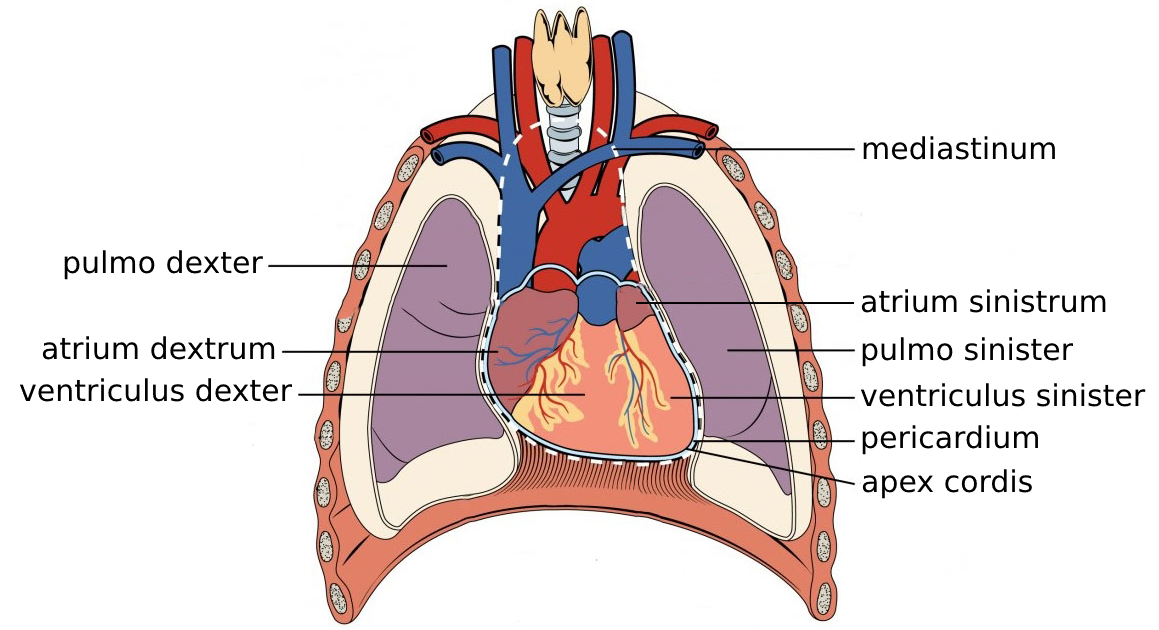
\includegraphics[width=0.7\textwidth]{../assets/anatomy/mediastinum}
		\caption{Umístění srdce v hrudní dutině mezi plícemi v mediastinu
			(Upraveno a převzato z \cite{OpenStax})}
		\label{fig:mediastinum}
	\end{center}
\end{figure}

\subsubsection{Struktura srdce}
\label{section:heart_structure}
Struktura srdce je tvořena dvěma síněmi (atrium dextrum et sinistrum) a dvěma
komorami (ventriculus dexter et sinister), oddělenými mezikomorovou přepážkou
(septum interventriculare), která současně rozděluje srdce na levé a pravé
\cite{Memorix2017}. O tok krve srdcem se starají čtyři srdeční chlopně,
fungující jako jednosměrné ventily, které jsou vidět na Obr.
\ref{fig:heartanatomy}, přičemž z komory pravého srdce je přečerpávána
neokysličená krev do plic. Z komory levého srdce se pumpuje okysličená krev do
celého krevního oběhu, a proto je svalovina levé komory silnější. Rozdíl zde
není jen ve svalovině ale také v krevním tlaku, jelikož pumpování krve do
tělního oběhu vyžaduje mnohem větší tlak než do plicního oběhu. Rozlišuje se
malý a velký oběh neboli krevní cirkulace pulmonální a systémová. Systematicky k
této cirkulaci dochází díky řetězci opakujících se elektrických a mechanických
událostí, uskutečněných během jedné časové periody, nazývané srdeční cyklus
(srdeční revoluce). Konkrétně se jedná o svalovou kontrakci (systola) a svalovou
relaxaci (diastola). Blíže je tento cyklus popsán v kapitole
\ref{section:cardiac_cycle}. Průtok krve srdcem je znázorněn pomocí bílých šipek
na ilustraci níže \cite{Stejfa2006}.

\begin{figure}[h]
	\begin{center}
		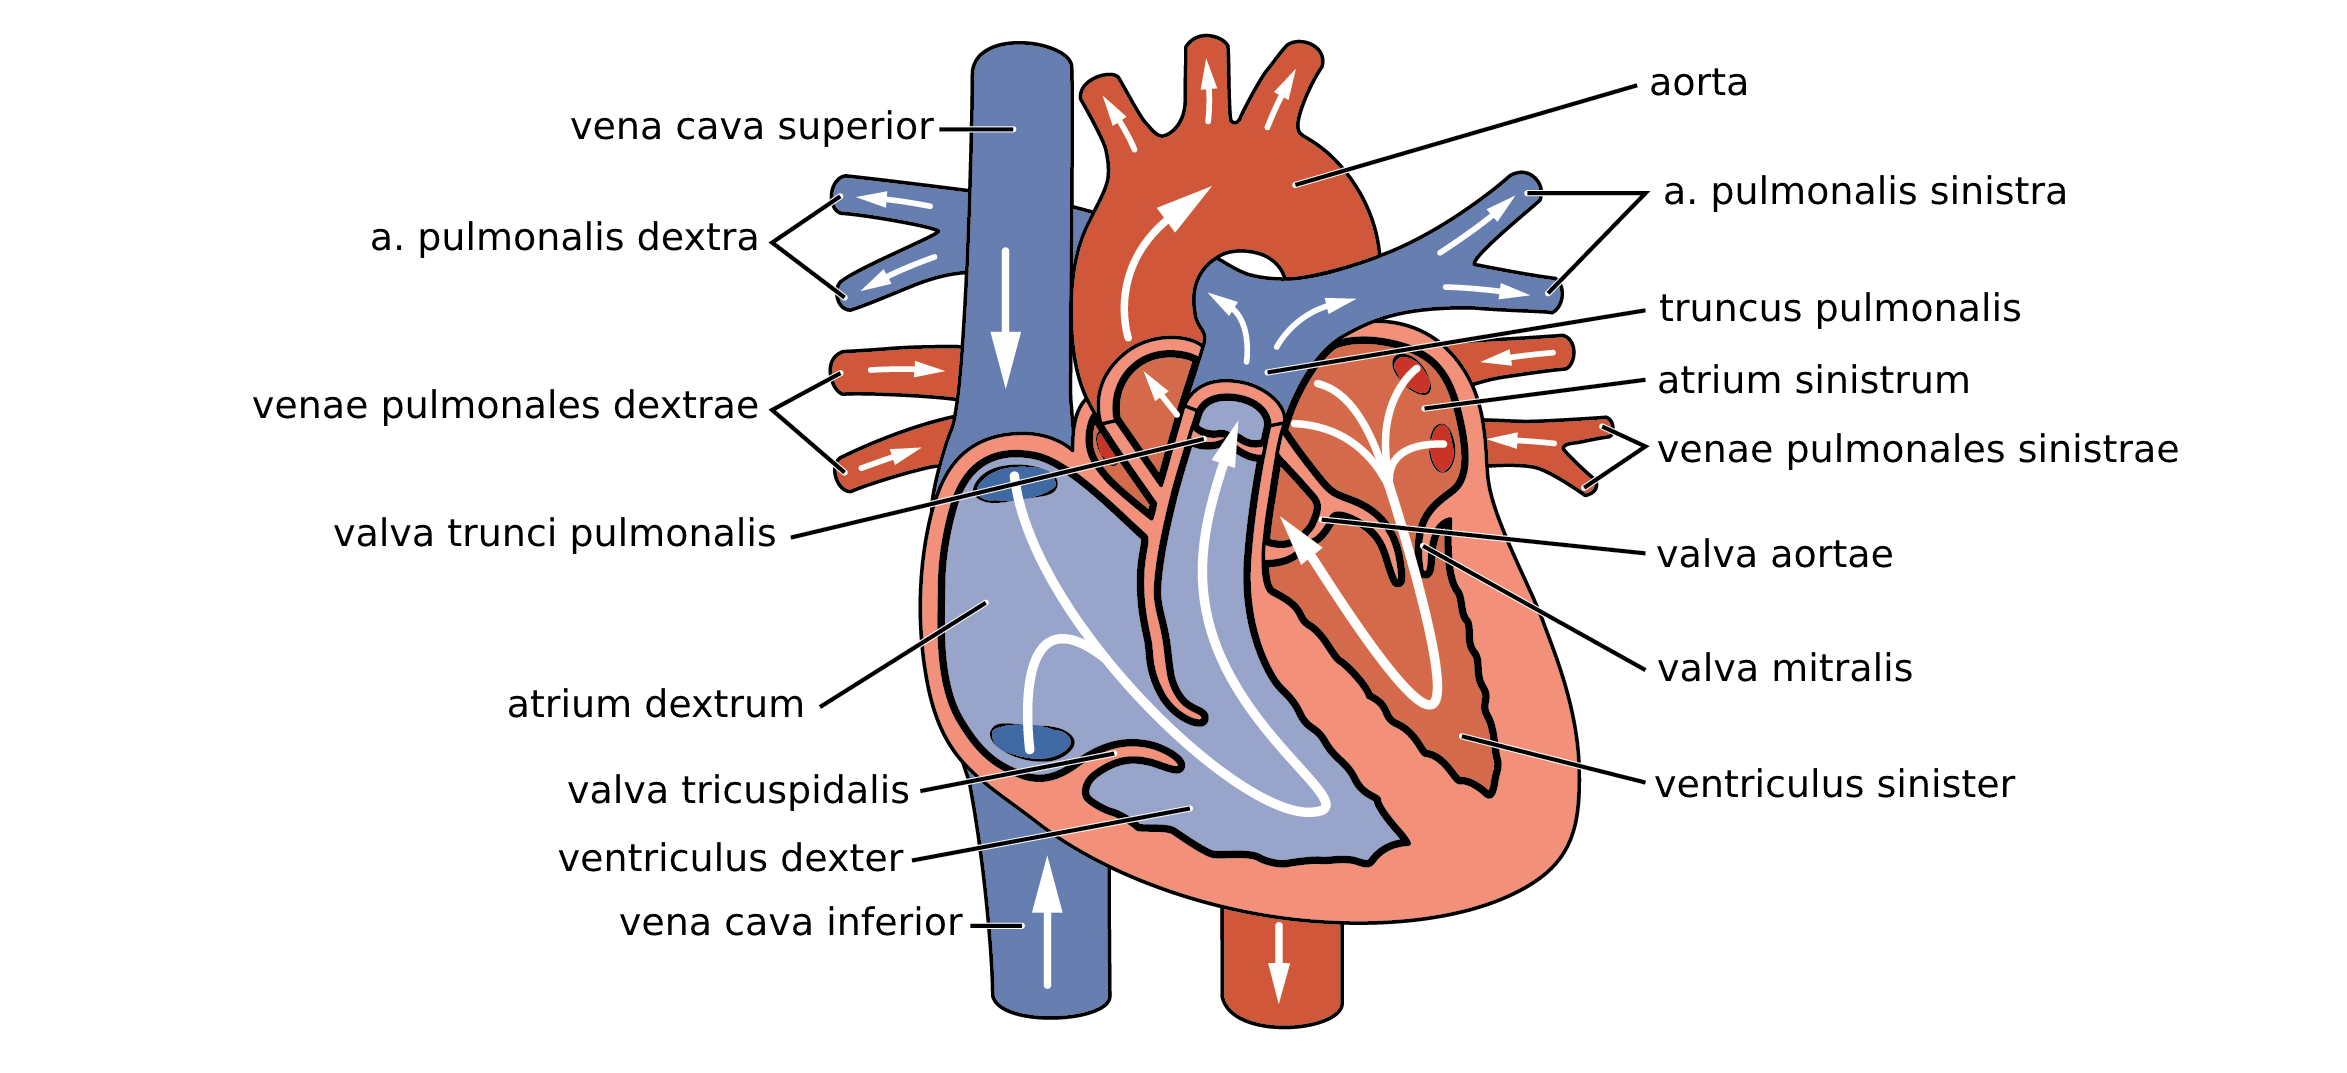
\includegraphics[width=1\textwidth]{../assets/anatomy/heart}
		\caption{Schéma srdce (anteriorní řez) zobrazující tok krve srdcem
			prostřednictvím bílých šipek (Upraveno a převzato z
			\cite{OpenStax})}
		\label{fig:heartanatomy}
	\end{center}
\end{figure}

Vnější část srdce, obdobně jako u cév, sestává ze tří vrstev: myokard (tunica
media), endokard (tunica intima) a epikard (tunica serosa), které společně tvoří
mohutný segment srdeční stěny \cite{Memorix2017}. Myokard (myocardium), nejširší
část srdeční stěny podléhající kontrakcím, je tvořen v závislosti na srdečním
oddílu dvěma až třemi vrstvami příčně pruhované svaloviny. Na myokard naléhá
silná řídká vrstva kolagenního vaziva a tuku neboli epikard (epicardium), ve
které probíhají cévy zásobující srdce. Poslední vrstvou, která vystýlá srdeční
dutiny a mezi síněmi a komorami tvoří mitrální chlopně, je endokrad
(endocardium). Povrch srdce obaluje vazivově-serózní blána, osrdečník
(pericardium). Prostor mezi perikardem a epikardem je vyplněn malým množstvím
serózní tekutiny, umožňující jejich vzájemný klouzavý pohyb, a nazývá se
perikardiální dutina (cavitas pericardialis) \cite{Weinhaus2005,Dylevsky2013}.

\begin{figure}[h]
	\begin{center}
		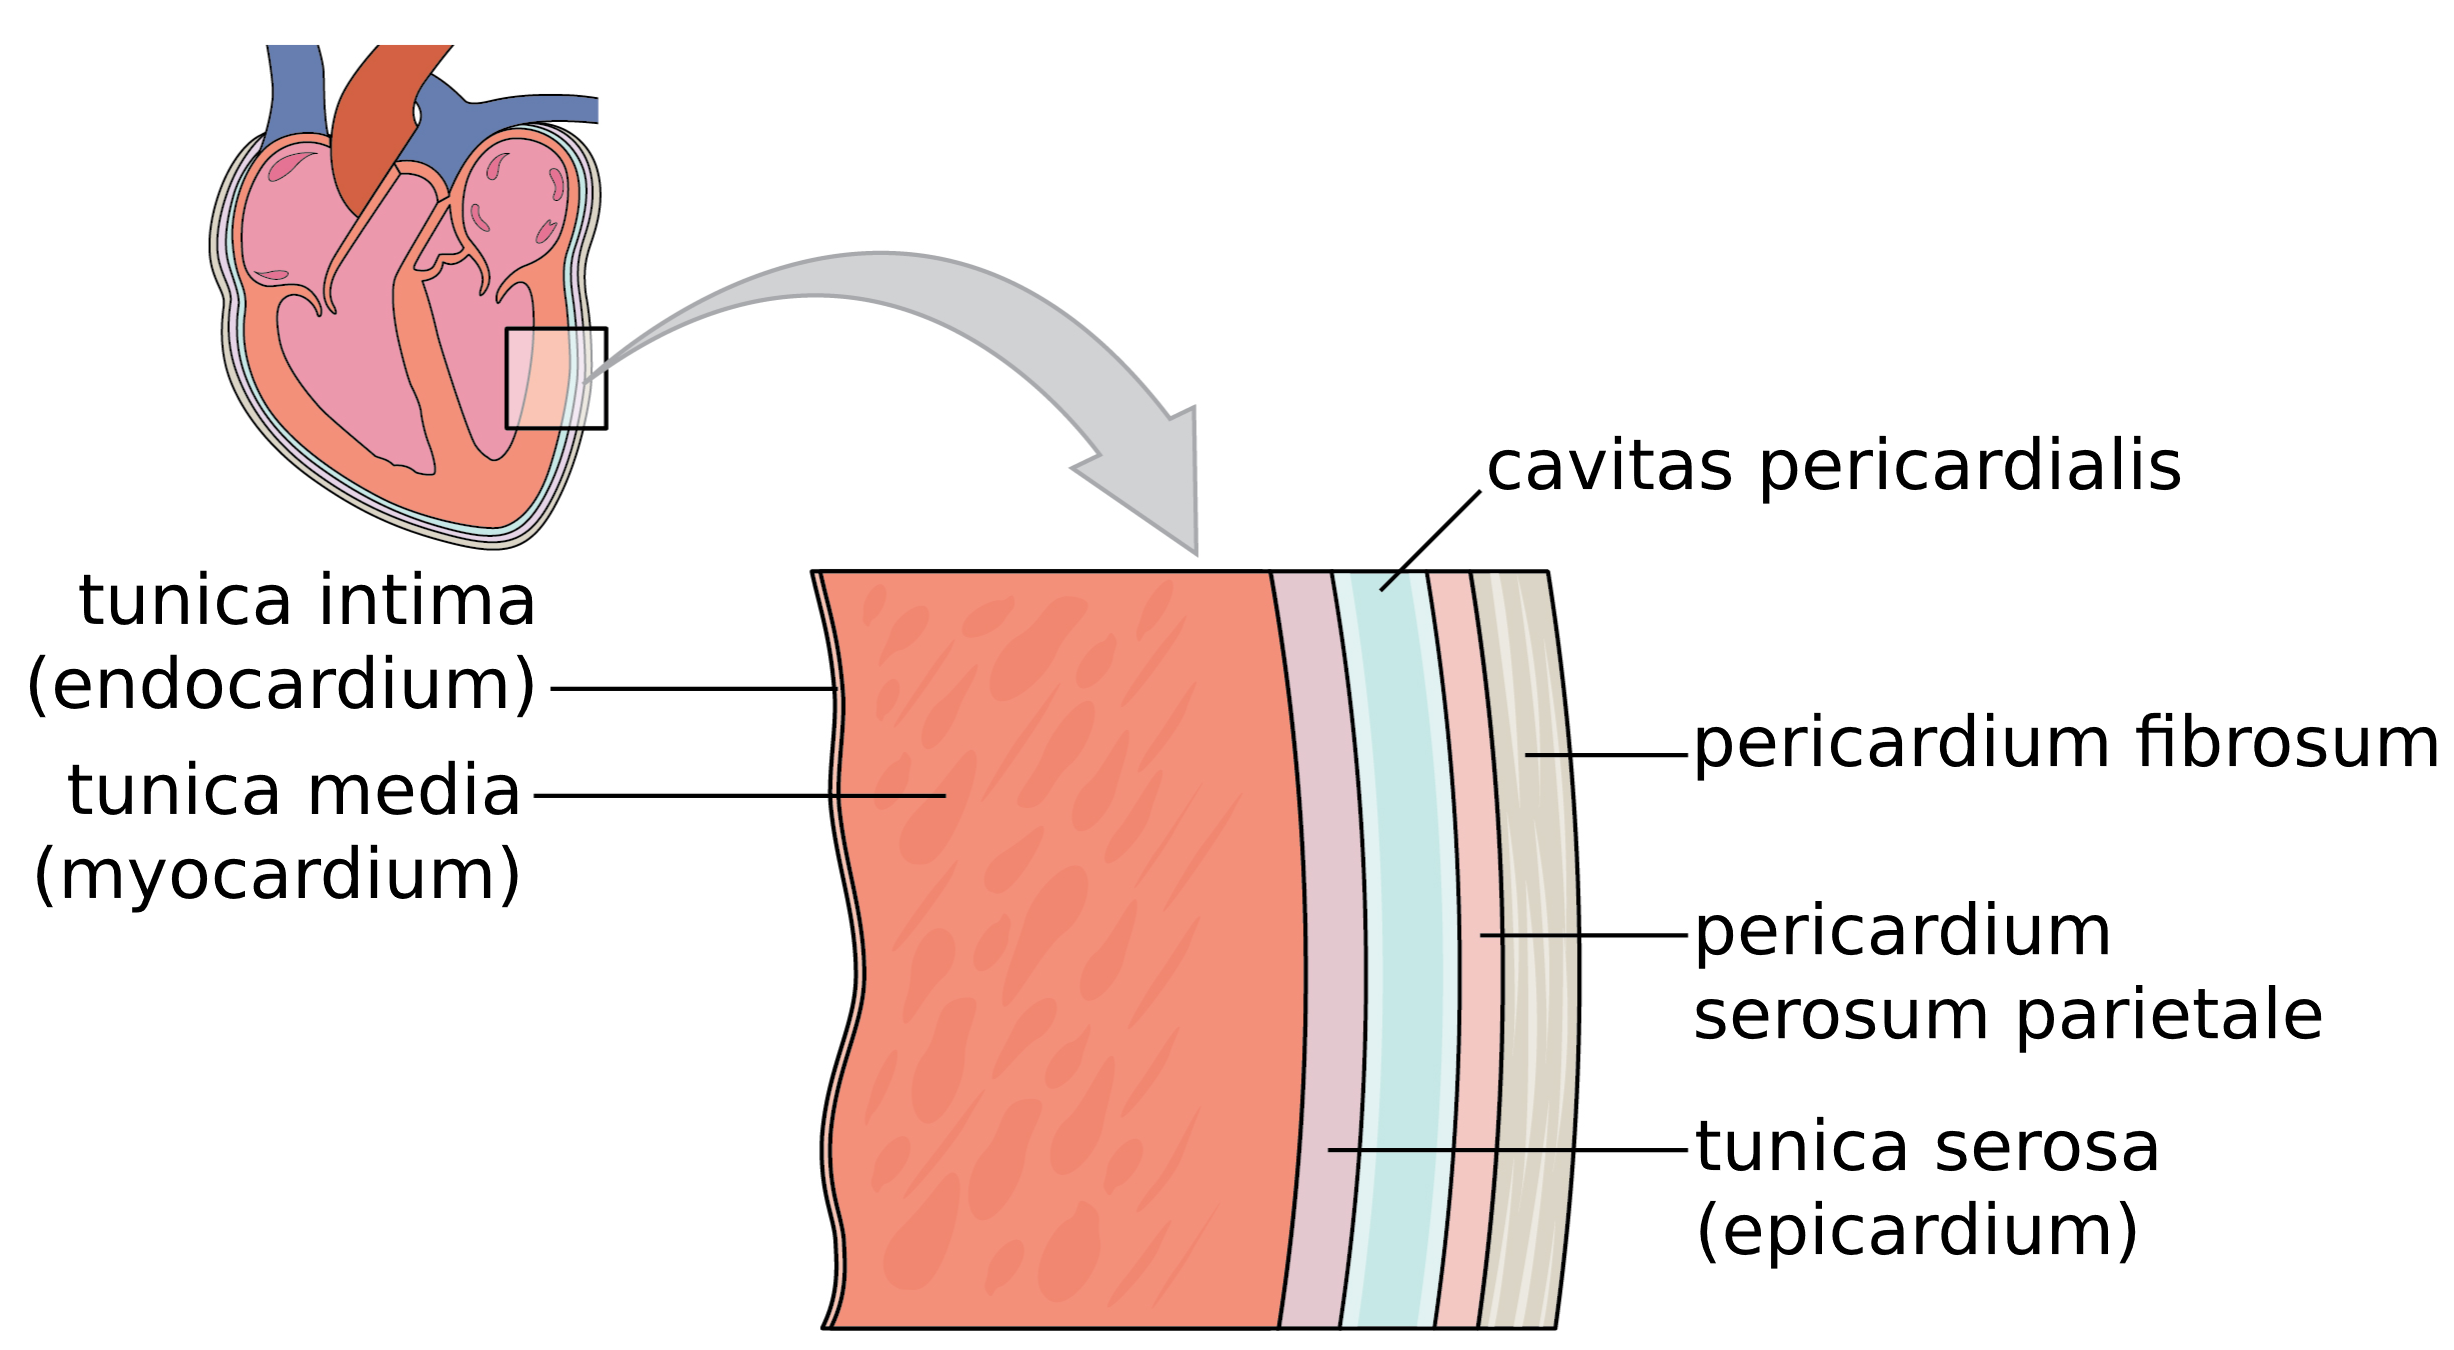
\includegraphics[width=0.7\textwidth]{../assets/anatomy/heart_muscle}
		\caption{Perikardiální membrána a vrstvy srdeční stěny (Upraveno a
			převzato z \cite{OpenStax})}
		\label{fig:heartlayers}
	\end{center}
\end{figure}

Obecně se srdeční svalovina skládá z příčně pruhované srdeční tkáně, avšak k
zajištění srdeční činnosti obsahuje kromě svalových buněk schopných kontrakce
(pracovní myokard) také specializované kardiomyocyty, tvořící převodní systém
srdeční (PSS). Tento systém společně ve spojení s autonomním nervovým systémem
(ANS) tvoří pro tuto práci zásadní část, a proto je podrobněji probrán v
samostatné kapitole \cite{Memorix2017,Dylevsky2013}.

\subsubsection{Srdeční cyklus}
\label{section:cardiac_cycle}
Jak již bylo naznačeno v kapitole \ref{section:heart_structure}, dvě z hlavních
funkcí srdce jsou: přečerpat neokysličenou krev ze systémového oběhu do plic,
kde dojde k její oxygenaci a pumpovat okysličenou krev z plic zpět do všech
tkání, kde dojde znovu k její deoxygenaci a celý proces se tak znovu opakuje.
Srdeční cyklus je tedy časově sladěný průběh dvou hlavních fází začínající
systolou a končící diastolou \cite{Weinhaus2005}. Systola je okamžik, kdy je ze
srdce kontrakcí a za vysokého tlaku vypuzována krev do oběhu, zatímco při
diastole neboli plnící nízkotlaké fází, se srdce krví plní. Síně i komory
podléhají oběma těmto fázím a jsou koordinovány otvíráním a zavíráním
atrioventrikulárních a semilunárních chlopní. Zároveň je regulována i čerpací
funkce srdce, tak aby v každém momentu byly splněny nároky tkání na okysličenou
krev \cite{OpenStax}. Detailněji jsou jednotlivé fáze srdečního cyklu popsány
níže.

\begin{figure}[h]
	\begin{center}
		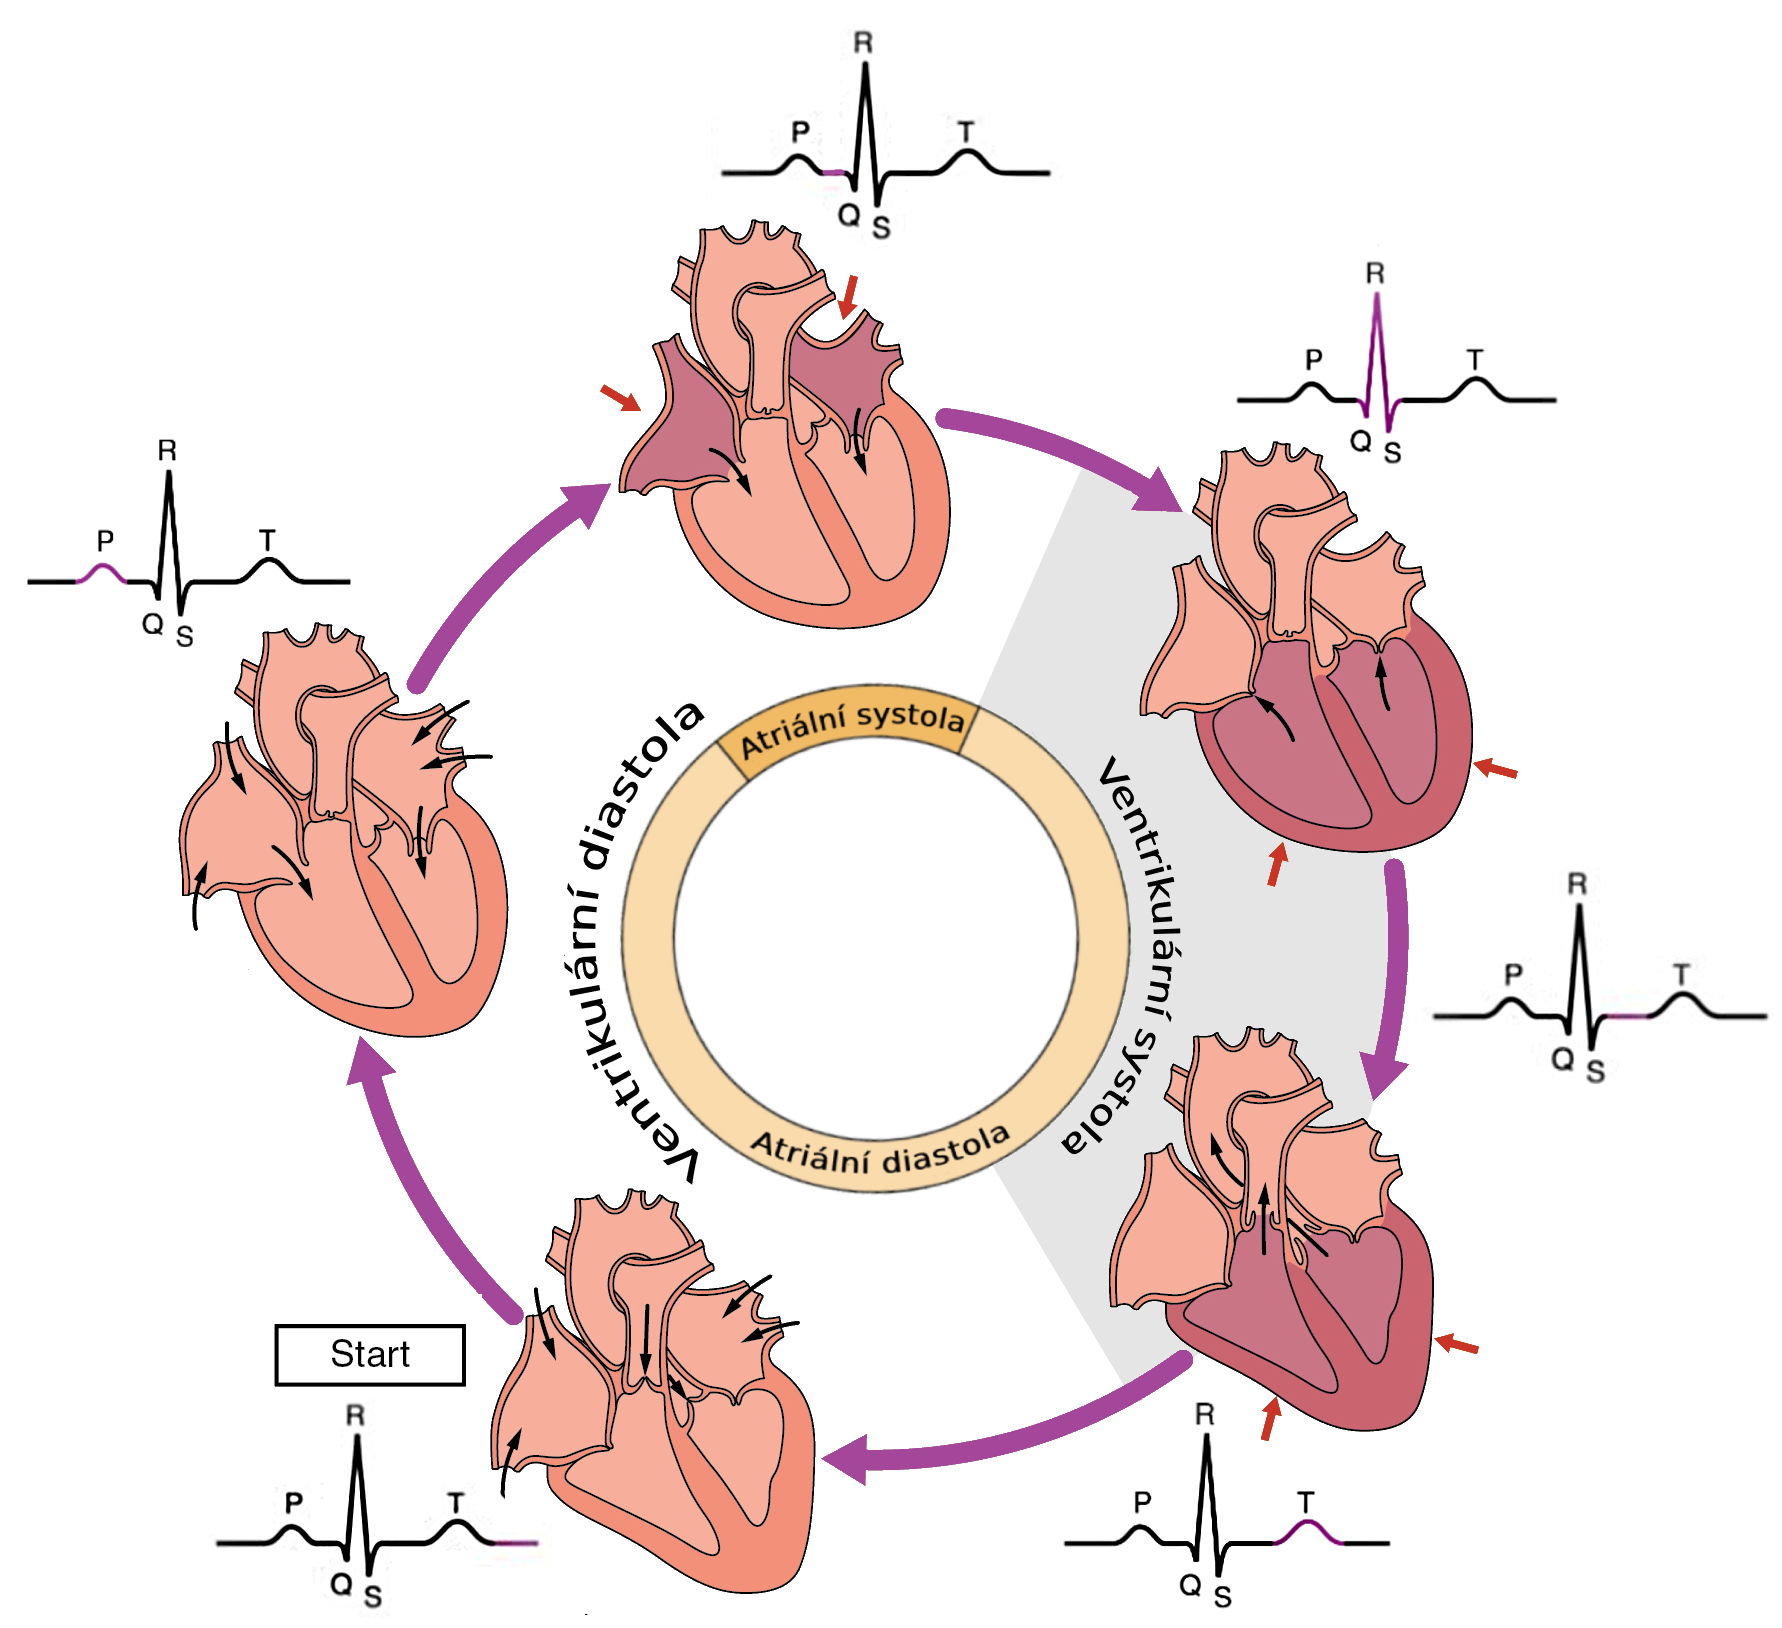
\includegraphics[width=0.9\textwidth]{../assets/anatomy/cardiac_cycle}
		\caption{Schéma srdečního cyklu (Upraveno a převzato z
			\cite{OpenStax})}
		\label{fig:cardiac_cycle}
	\end{center}
\end{figure}

\paragraph*{\textit{Plnící fáze (atriální diastola)}\\} Síně a komory jsou
relaxované. Komory srdce se pod nízkým tlakem (0--10 \si\mmHg) plní
neokysličenou krví přicházející ze systémového oběhu. Krev proudí do levé síně z
venae cave inferior et superior a sinus coronarius. Do lévé síně přichází krev z
plicních žil. Otevřenou trikuspidalní a mitrální chlopní proudí krev dál ze síní
právě do komor. Komory se naplní krví přibližně do 70--80 \% jejich kapacity
\cite{OpenStax}.

\paragraph*{\textit{Izovolumická fáze (atriální systola)}\\} Síně podléhají
kontrakci a zvyšuje se v nich tlak. Díky tomu je do komor otevřenými
atrioventrikulárními chlopněmi dopraveno zbylých 20--30 \% krve. Kontrakce síní
je podmíněna depolarizací, kterou na EKG reprezentuje P vlna a trvá přibližně
100 \si\ms. Konec fáze je doprovázen otevřením semilunárních chlopní
\cite{OpenStax}.

\paragraph*{\textit{Ejekční fáze (ventrikulární systola)}\\} Tlak v komorách
roste následkem jejich kontrakce, dokud není dostatečně velký, aby došlo k
otevření semilunárních chlopní. Krev je pak vypuzena z komor do tepen, přičemž v
komorách vždy zůstává konečný systolický objem (end systolic volume, ESV) krve,
který činí přibližně 50--60 \si\ms. Ventrikulární systola je podmíněna
depolarizací komor, která je na EKG záznamu reprezentovaná jako QRS komplex.
Tato fáze trvá přibližně 270 \si\ms \cite{OpenStax}.

\paragraph*{\textit{Fáze izovolumické relaxace (ventrikulární diastola)}\\}
Ventrikulární relaxace je doprovázená repolarizací komor a na EKG reprezentovaná
T vlnou. Trvá přibližně 430 \si\ms. Komory přecházejí do stavu relaxace a tlak v
nich klesá až dojde ke zavření semilunárních chlopní. Tlak v komorách poté klesá
dále, než klesne pod hodnotu tlaku v síních. Krev začíná proudit ze síní do
komor, což má za následek otevření trikuspidalní a mitrální chlopně. Obě komory
přecházejí do diastoly \cite{OpenStax}.

\subsubsection{Převodní systém srdeční}
\label{section:pss}
Anatomicky se tento systém skládá ze sinoatriálního uzlu (SA uzel, nodus
sinoatrialis), atrioventrikulárního uzlu (AV uzel, nodus atrioventricularis),
síňokomorového svazku (Hisův svazek, fasciculus atrioventricularis) s jeho
raménky (Tawarova raménka, crus dextrum et sinistrum fasciculi
atrioventricularis) a koncovými vlákny (Purkyňova vlákna, rami subendocardiales)
končicími ve svalovině komor. Tato stavba je vyznačena na Obr. \ref{fig:pss}
\cite{Dylevsky2013}.

\begin{figure}[h]
	\begin{center}
		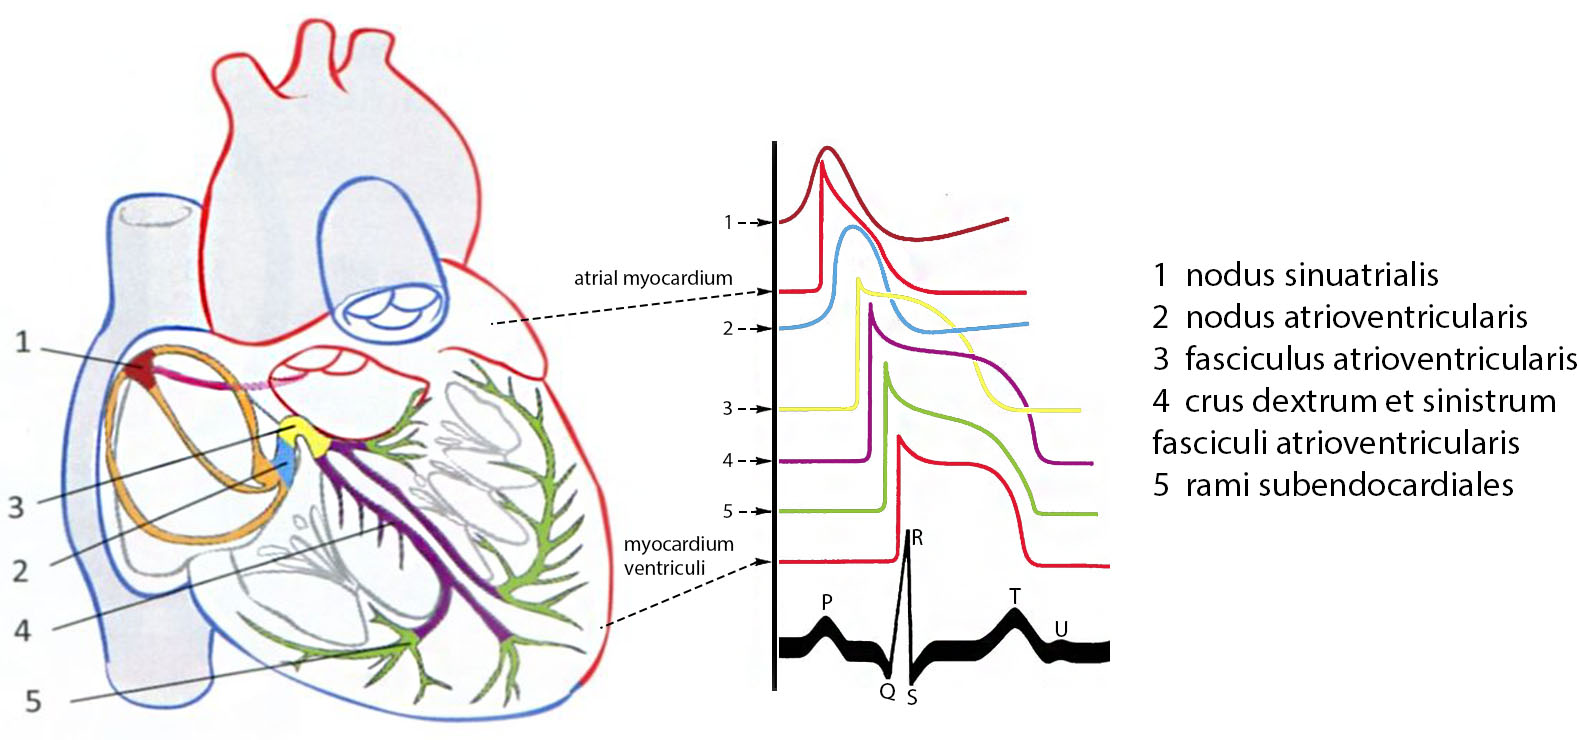
\includegraphics[width=0.9\textwidth]{../assets/anatomy/pss}
		\caption{Převodní systém srdeční (Upraveno a převzato z
			\cite{ecgpediaConduction})}
		\label{fig:pss}
	\end{center}
\end{figure}

Z funkčního hlediska se jedná o soubor specializovaných částí myokardu. První
část tvoří buňky pracovního myokardu, jejichž hlavním úkolem je kontrakce
\cite{Cihak2016}. Druhou část reprezentují specializované buňky převodního
srdečního systému --- kardiomyocyty --- které jsou morfologicky těžko
odlišitelné, avšak funkčně, na rozdíl od buněk pracovního myokardu mají na
starosti autonomní generaci akčního potenciálu (AP) a rychlé vedení vzruchu
elektrického charakteru za účelem podráždění myokardu (excitabilita) a vyvolání
jeho stahu (systola). Ke vzniku těchto vzruchů dochází uvnitř orgánu (automacie)
a poté se šíří dále. 

Navzájem jsou propojeny interkalárními disky (disci intercalares), jejichž
součástí jsou \textit{gap junctions} neboli specializované struktury zajišťující
převod impulsu mezi kardiomyocyty. V místech, kde toto propojení nevzniká jsou
spoje mezi jednotlivými buňkami zajištěny desmozomy a nexy umožňující jejich
vzájemnou komunikaci \cite{Dylevsky2013, Stejfa2006}.

Srdce, konkrétně srdeční svalovinu (myokard) spolu s PSS tedy charakterizuje
několik hlavních funkcí \cite{Stejfa2006}:
\begin{itemize}
	\item \textit{Automacie (chronotropie, samočinnost)} --- samočinná rytmická
	      generace elektrických impulzů pacemakerovými buňkami k podnícení
	      pravidelné kontrakce.
	\item \textit{Excitabilita (bathmotropie, dráždivost)} --- reakce na
	      podráždění elektrickým impulzem depolarizací.
	\item \textit{Konduktivita (dromotropie, vodivost)} --- vedení vzniklých
	      elektrických vzruchů celou srdeční svalovinou.
	\item \textit{Stážlivost (inotropie, kontraktilita)} --- mechanická odpověď
	      kontraktilních buněk pracovního myokardu na vzniklé elektrické
	      podněty.
\end{itemize}

V zmíněných dvou funkčních částech je také potřeba rozlišovat rozdíly na buněčné
úrovní, a to konkrétně v rámci membránových potenciálů.

Buňky pracovního myokardu sice za normálních podmínek ve zdravém srdci
nevyužívají schopnost samovolně vytvářet vzruchy ale jejich dráždění vyvolává
šíření akčního potenciálu napříč myokardem, což má za následek zahájení
kontrakce. Jejich klidový membránový potenciál se pohybuje okolo -90 mV. Změnou
klidového membránového potenciálu vzniká akční potenciál, jehož časový průběh
sestává z následujících fázi: rychlá depolarizace (fáze 0), časná repolarizace
(fáze 1), plató akčního potenciálu (fáze 2), konečná repolarizace (fáze 3) a
návrat ke klidovému potenciálu (fáze 4) \cite{Petrek2019}.

\begin{figure}[h]
	\centering
	\begin{subfigure}{0.4\textwidth}
		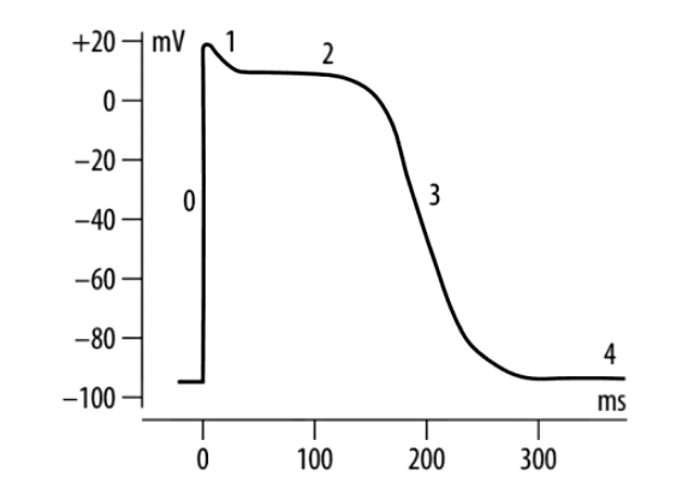
\includegraphics[width=1\textwidth]{../assets/anatomy/myokard_ap}
		\caption{Akční potenciál buňky pracovního myokardu \cite{Petrek2019}}
		\label{fig:myokard_ap}
	\end{subfigure}
	\hfil
	\begin{subfigure}{0.5\textwidth}
		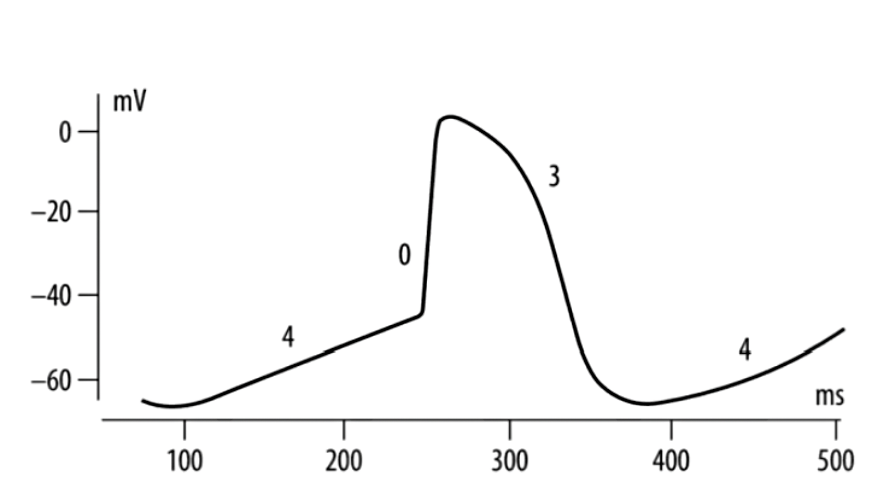
\includegraphics[width=1\textwidth]{../assets/anatomy/pss_ap}
		\caption{Akční potenciál buňky převodního systému srdce
			\cite{Petrek2019}}
		\label{fig:pss_ap}
	\end{subfigure}
	\caption{Rozdíl průběhů akčních potenciálu pracovního myokardu a převodního
		systému srdce: 0 --- rychlá depolarizace, 1 --- časná repolarizace, 2
		--- plató akčního potenciálu, 3 --- konečná repolarizace, 4 --- návrat
		ke klidovému potenciálu}
	\label{fig:ap}
\end{figure}

Klidový membránový potenciál pacemakerových buněk --- buněk SA a AV uzlu --- je
více depolarizován, než u buněk pracovního myokardu (-50 až -70 mV) a samovolně
klesá k prahové hodnotě (spontánní diastolická depolarizace). Jakmile klidový
potenciál dosáhne prahové hodnoty vzniká další akční potenciál. Průběh akčního
potenciálu se od buněk pracovního myokardu také liší. Chybí zde 1. a 2. fáze.
Grafy akčních potenciálů jsou na Obr. \ref{fig:ap} \cite{Petrek2019}.

Elektrické vzruchy, vyvolávající rytmické smršťování srdečního svalu, primárně
vznikají v SA uzlu, uloženém při ústí horní duté žíly, ve stěně pravé síně.
Tento uzel je udavatel srdečního rytmu (HR) neboli primární pacemaker a vzruchy
se z něj šíří dále systémem. Než jsou tyto impulzy převedeny přes Hisův svazek
na Purkyňova vlákna, prochází vzruch AV uzlem (sekundární pacemaker), kde
dochází k jeho zpomalení a tvorbě časové prodlevy, což má za následek postupné
kontrakce síní a komor. Spojení mezi SA uzlem a AV uzlem je realizováno
internodálními síňovými spoji, což jsou vlákna stejného charakteru jako u PSS.
Tyto spoje umožňují rozvádět vzruchy z SA uzlu rychleji než samotná svalovina
síní. Vzruchy je pak možno mezí síněmi a komorami vést pomaleji či rychleji, což
představuje jeden z regulačních mechanismů srdeční frekvence
\cite{Dylevsky2013,Cihak2016}.

Tento sled, pravidelnost srdečního rytmu a proměnlivost srdečních akcí vůči
změnám v organismu, zajišťuje několikastupňový regulační systém. Zachycením
těchto elektrických potenciálů v čase spolu se změnami jejich potenciálu vzniká
tzv. elektrokardiogram (EKG), na kterém je zachycen průběh elektrického
srdečního cyklu s jeho jednotlivými fázemi (Obr. \ref{fig:pss} --- P, Q, R, S,
T, U) \cite{Dylevsky2013,Cihak2016}.


\subsubsection{Regulace srdeční frekvence}
\label{section:hr_regulation}
Změny v srdeční frekvenci (chronotropie) a její variabilitě jsou jedním z
následků regulace srdeční činnosti, která mimo jiné ovliňuje také inotropii,
dromotropii a bathmotropii. Regulaci se dělí na dvě úrovně v závislosti na místě
průběhu regulačního děje, a to na intrakardiální a extrakardiální.
Intrakardiální regulační děje probíhají v srdci samotném, například následkem
mechanických změn myokardu. Blíže tyto děje popisuje například Starlingův zákon
nebo Bainbridgeův reflex \cite{Kittnar2020}. Extrakardiální děje se dělí dále na
nervové a humorální. Jelikož je srdeční frekvence řízena hlavně nervově, tak se
tato kapitole věnuje podrobněji extrakardiálním vlivům \cite{Orel2019}.

\paragraph*{\textit{Nervová regulace srdečního rytmu}\\} Srdce je inervováno
autonomním (vegetativním) nervovým systémem, konkrétně pregangliovými
parasympatickými vlákny (rami cardiaci nervi vagi) z bloudivého nervu (nervus
vagus) a sympatickými vlákny z krčního kmene sympatiku (n. cardiacus cervicalis
superior, medius et inferior), společně s větvemi jeho horního hrudního úseku
(nn. cardiaci thoracici) \cite{Dylevsky2013,Kittnar2020}. Tato vlákna realizují
regulační děje, vzniklé na úrovní prodloužené míchy (medulla oblongata) v
kardioexcitačním nebo kardioinhibičním centru. Inervace tohoto typu představují
jeden z vyšších stupňů regulačních mechanismů a jejich dráždění má vliv na
srdeční frekvenci a její variabilitu \cite{Dylevsky2013,Trojan2002}.

\begin{figure}[h]
	\begin{center}
		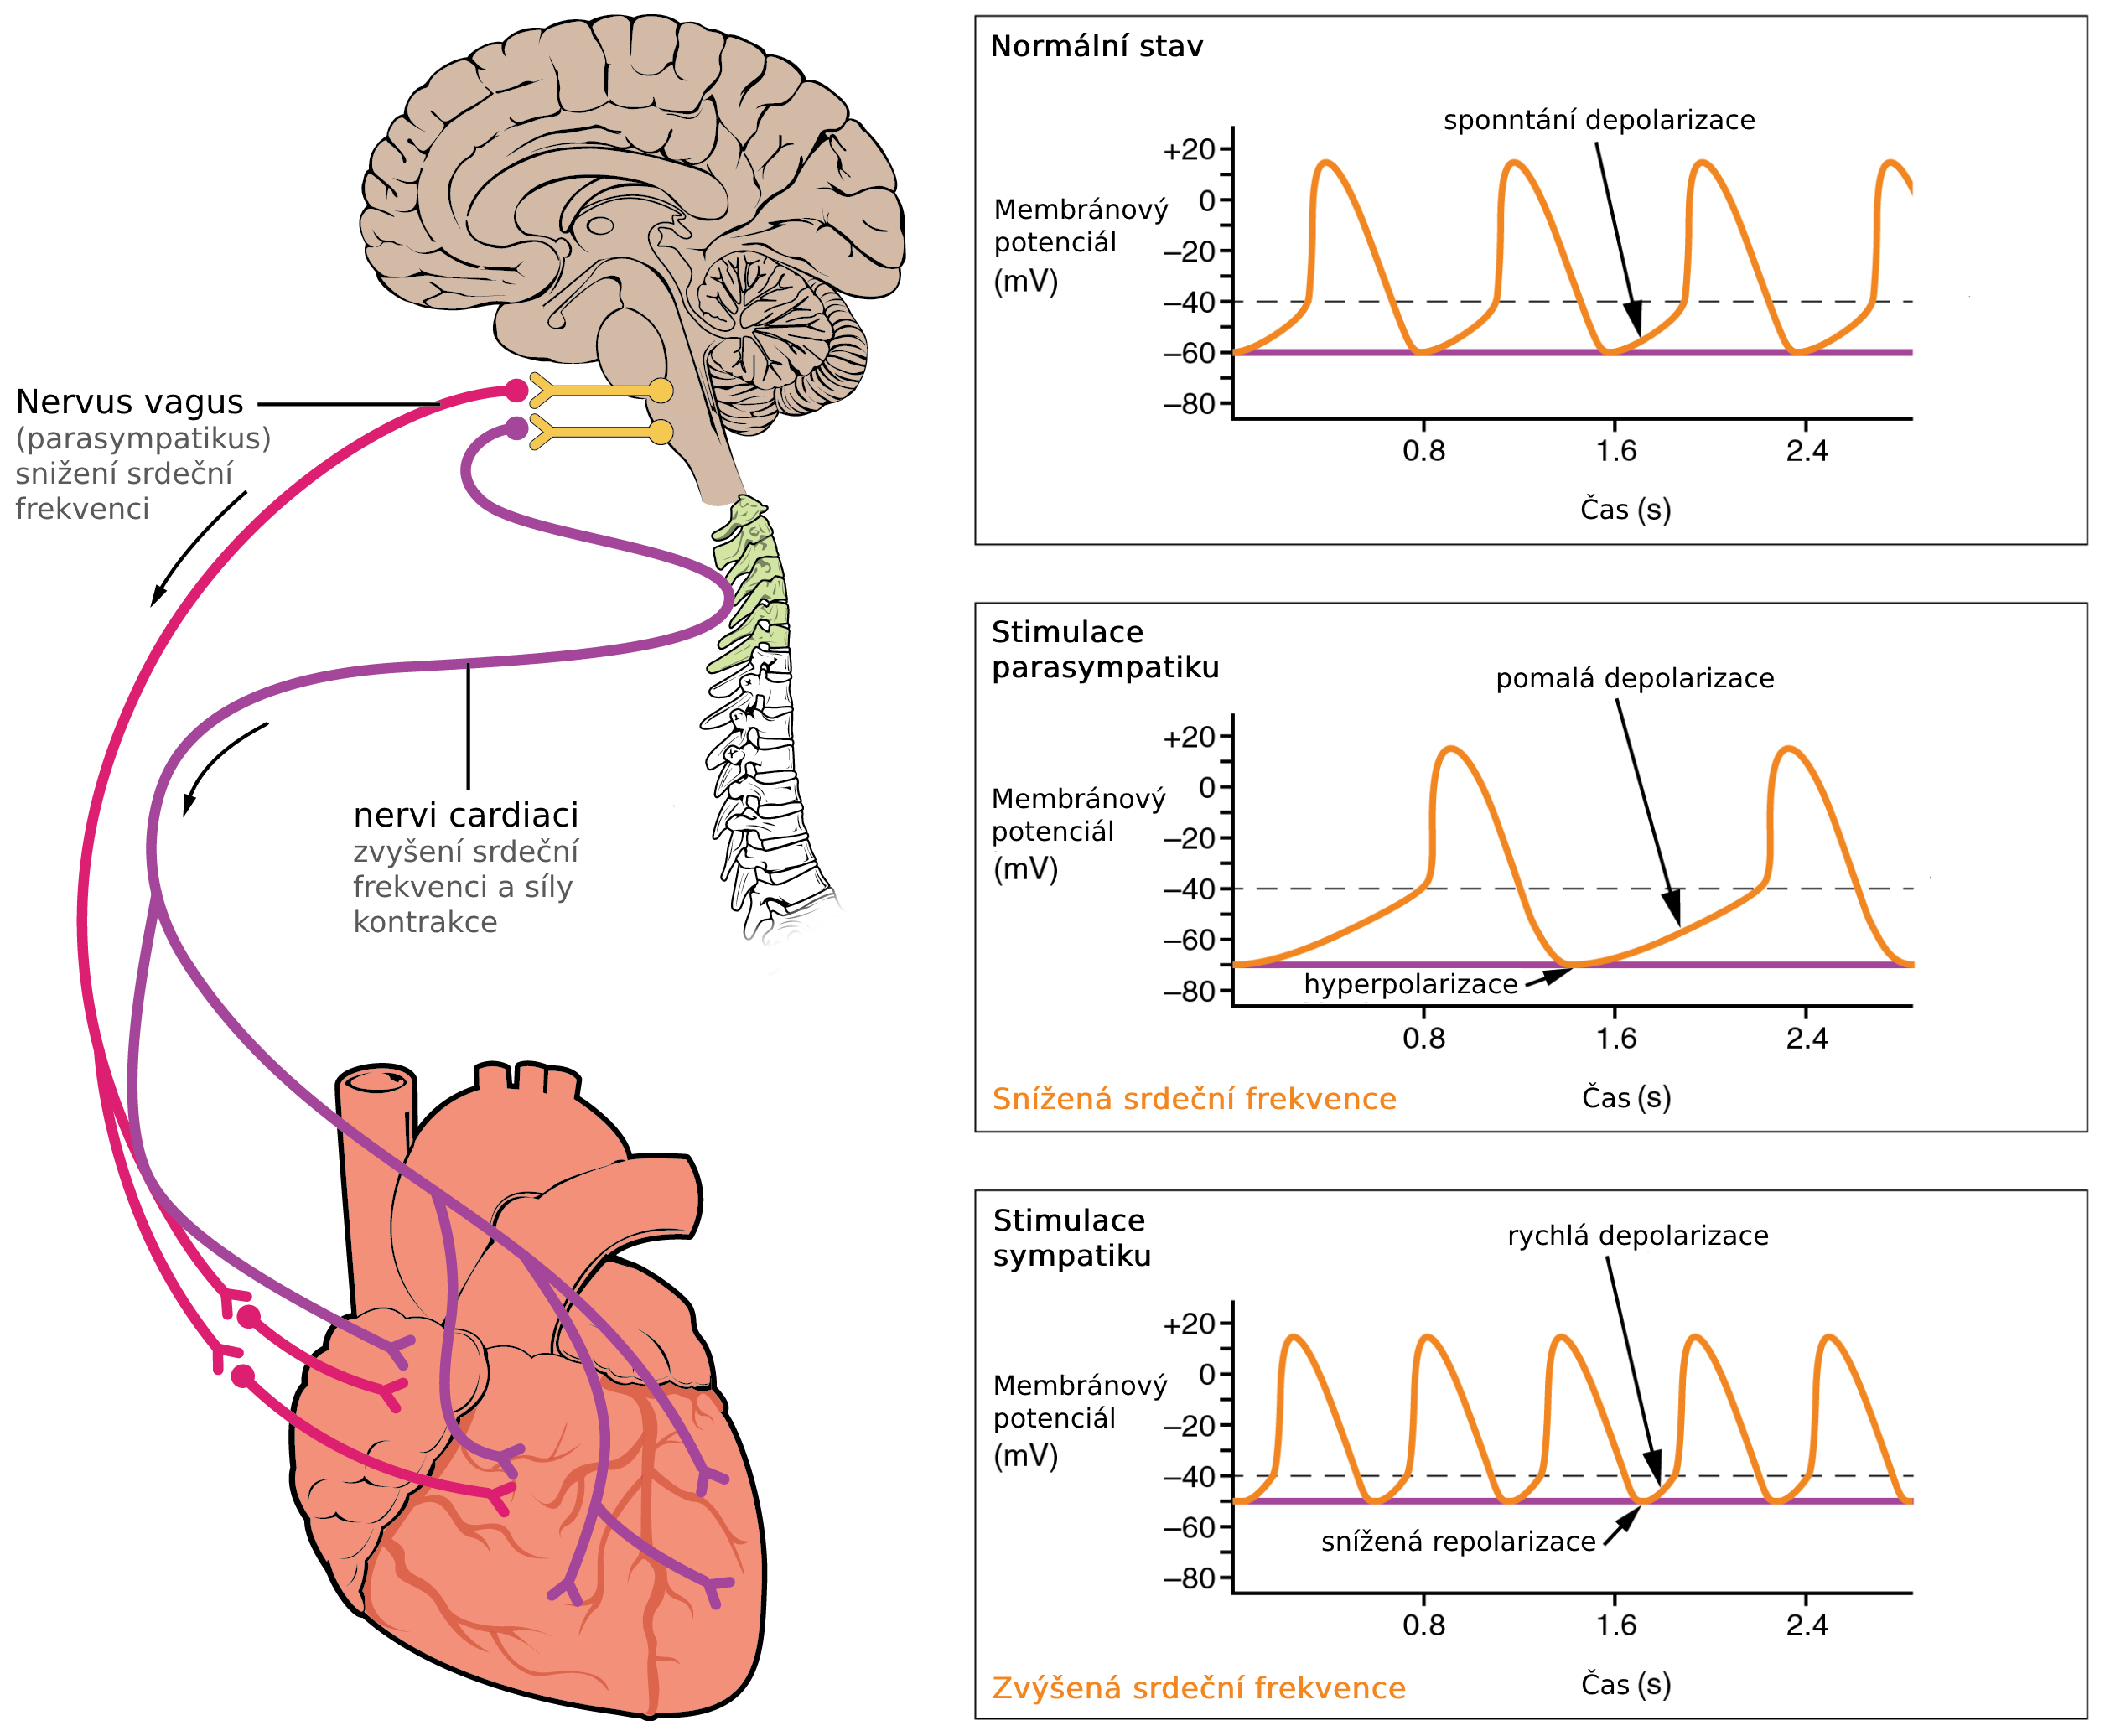
\includegraphics[width=1\textwidth]{../assets/anatomy/hr_regulation}
		\caption{Autonomní invervace kardioexcitačních a kardioinhibičních
			oblastí nacházejících se v prodloužené míše a jejich vliv na
			normální sinusový rytmus (Upraveno a převzato z \cite{OpenStax})}
		\label{fig:hr_regulation}
	\end{center}
\end{figure}

Srdeční odezva na tyto nervové podněty je realizována na nejnižší intrakardiální
úrovní pomocí srdečních ganglií, které se skládají z neuronů. Přesněji jsou to
hlavně cholingerní (vagální) a adrenergní (sympatické) srdeční neurony, sloužící
jako vagální spínací body se schopností reakce na chemické, mechanické a
elektrofyziologické podněty. Díky tomu může například nervová aktivita v
prefrontální kůře modulovat HRV (\ref{section:hrv}). Blíže tyto vztahy popisuje
model Neuroviscerální integrace (NVI) \cite{Smith2017}.

Vliv parasympatiku je realizován uvolňováním mediátoru --- acetylcholinu --- z
koncových postgangliových vláken. Odpověď probíha v srdeční tkání díky
muskarinovým cholingerním recepotorům. Stimulací těchto receptorů se zpomaluje
proces spontánní diastolické depolarizace. To má za následek nižší srdeční
frekvenci (negativní chronotropie) v SA uzlu a zpomalení síňokomorového převodu
vzruchů v AV uzlu. Obecně stimulace parasympatiku způsobuje včetně zpomalení HR
a síňokomorového převodu také snížení srdeční kontrakce a excitability myokardu
\cite{Kittnar2020}.

Stimulací sympatiku nastávají přesně opačné účinky než u parasympatiku. Ty
zahrnují zrychlení HR a síňokomorového převodu spolu se zvýšenou excitabilitou a
silou kontrakcí myokardu. Mediátorem je zde noradrenalin, který v
kardiomyocytech aktivuje \textbeta-adrenergní receptory, což vyvolává zrychlenou
spontánní depolarizaci. Výsledkem je primárně již zmíněná zvýšená srdeční
frekvence \cite{Kittnar2020}.

\paragraph*{\textit{Humorální regulace srdečního rytmu}\\} Regulace na této
úrovni vzniká vlivem hormonů, a to především působením katecholaminů ---
adrenalin a noradrenalin ---, produkovaných dření nadledvin nebo adrenergními
neurony sympatiku. Mají okamžitý nástup účinků, které jsou podobné těm jako u
stimulace sympatiku. Mezi další hormony ovlivňující srdeční frekvenci patří také
například hormony štítné žlázy, tyroxin a trijodthyronin
\cite{Kittnar2020,Orel2019}.

\paragraph*{\textit{Další faktory regulující srdeční rytmus}\\} Dalšími vlivy,
které ovlivňují srdeční frekvenci jsou například: koncentrace různých
elektrolytů v těle, tělesná teplota, rovnováha pH, dýchání, fyzická zátěž nebo
různé druhy kognitivní zátěže. Dále změny krevního tlaku, na které jsou citlivé
baroreceptory umístěné v oblouku aorty (arcus aortae) neboli tzv. reflexní
řízení. Mimo jiné se tato frekvence liší i věkem, pohlavím či zdravotními
podmínkami \cite{Kittnar2020}.

\subsection{Elektrokardiografie}
\label{section:electrocardiography}
Jednou z nejčastějších neinvazivních diagnostických metod v klinické praxi,
hlavně v oblasti kardiologie, je záznam a interpretace elektrické aktivity srdce
neboli elektrokardiografie. Princip této metody spočívá v měření elektrických
projevů srdeční aktivity na povrchu lidského těla. Každá perioda srdečního cyklu
je na buněčné úrovní doprovázená genezí nerovnoměrného elektrického napětí (AP),
což má za následek vznik místních elektrických proudů, resp. elektrického pole v
okolí myokardu \cite{Kittnar2020}. Vzniklé elektrické pole je zde ve skutečnosti
součtem jednotlivých elektrických polí každé srdeční buňky, kterou je možno
vyjádřit elementárním vektorem. Elementární vektory vyjadřují velikost a směr
elektrického pole \cite{Stejfa2006}. Sumací vektorů v jednom časovém momentu
vzniká okamžitý vektor elektrického pole jehož orientace a velikost
charakterizují výslednou naměřenou amplitudu v specifickém svodu, viditelnou na
EKG křivce \cite{Surawicz2008,Kittnar2020}.

Tkáně v lidském těle díky jejich elektrickým vlastnostem plní při styku s
elektrickým polem úlohu vodiče, což umožňuje naměřit napětí mezi různými místy
na povrchu těla. K snímaní napětí na rozhraní kůže se používají elektrody.
Zaznamenáváním výsledné hodnoty naměřených rozdílů potenciálu mezi elektrodami v
čase vzniká tzv. elektrokardiogram. Měření se liší počtem použitých svodů a
jejich lokalizací na lidském těle. Elektrokardiografie se kategorizuje z
hlediska počtu, zapojení a umístění svodů do těchto základních skupin:
\cite{Haberl2012,Kittnar2020}:

\begin{enumerate}
	\item \textbf{Einthovenovy bipolární končetinové svody (I, II, III)} ---
	      vytváří tzv. teoretický Einthovenovův rovnoramenný trojúhelník, jehož
	      přibližným středem je srdce. Elektrody se v tomto případě většinou
	      nachází na horních končetinách a levé dolní končetině, přičemž dvě z
	      nich jsou elektrody aktivní. Měřenou amplitudu udává rozdíl potenciálu
	      aktivních elektrod. Tyto svody jsou často nazývané standardními
	      \cite{Kittnar2020}.
	      \begin{figure}[h]
		      \begin{center}
			      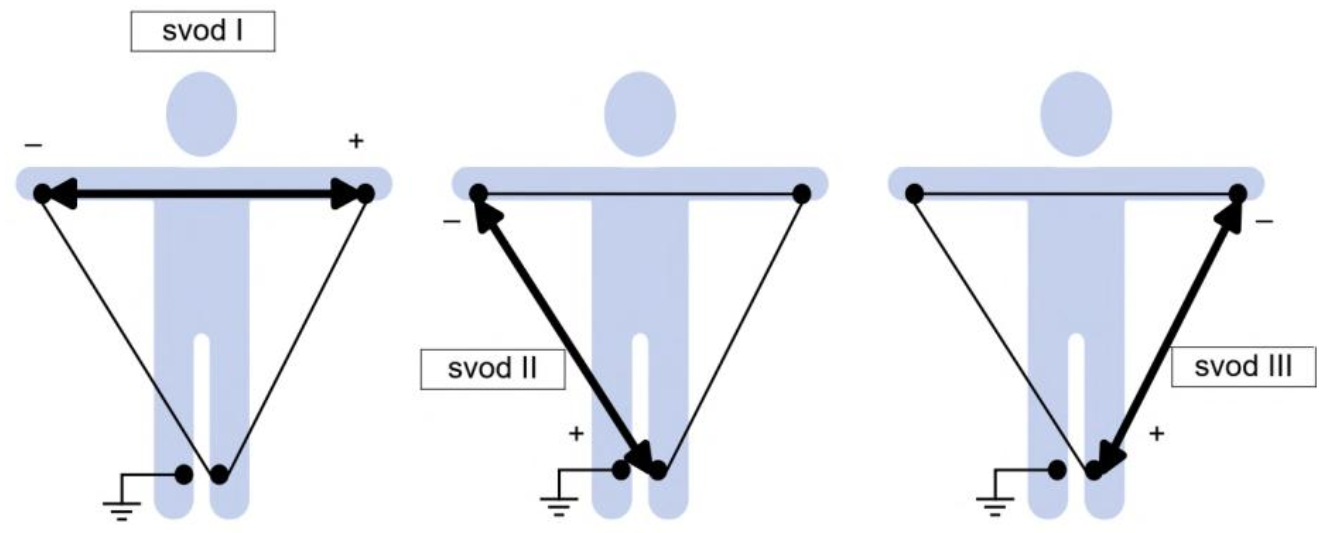
\includegraphics[width=0.75\textwidth]{../assets/anatomy/bipolar}
			      \caption{Bipolární končetinové svody \cite{Kittnar2020}}
			      \label{fig:bipolar}
		      \end{center}
	      \end{figure}
	\item \textbf{Goldbergerovy unipolární končetinové svody (aVR, aVL, aVF)}
	      --- původně tvořily spoje aktivních elektrod s Wilsonovou virtuální
	      svorkou. K Wilsonově svorce byly připojeny všechny končetinové svody
	      přes vyoský odpor ke zajištění nulového potenciálu na této svorce.
	      Pozdějí byl tento způsob upraven Goldbergerem, který touto modifikací
	      zesílil amplitudu svodů na záznamu. Zesílení vzniká odpojením aktivní
	      elektrody od Wilsonovy svorky čimž je následně měřen potenciál pouze
	      mezi odpojenou elektrodou a zbylými \cite{Kittnar2020}.
	      \begin{figure}[h]
		      \begin{center}
			      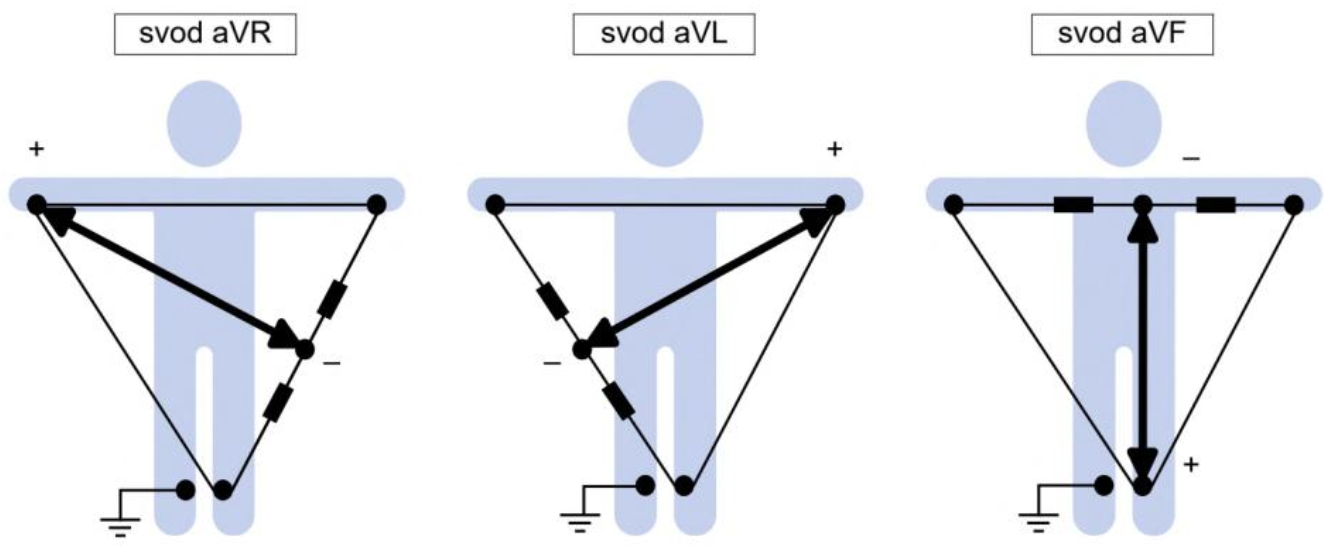
\includegraphics[width=0.75\textwidth]{../assets/anatomy/unipolar1}
			      \caption{Unipolární končetinové svody \cite{Kittnar2020}}
			      \label{fig:unipolar1}
		      \end{center}
	      \end{figure}
	\item \textbf{Wilsonovy unipolární hrudní svody (V1 -- V6)} --- sestávají z
	      šesti hrudních elektrod zapojených proti referenční Wilsonově svorce.
	      Wilsonova nulová svorka je zde opět tvořená spojením končetinových
	      svodů přes odpor. Změnou v tomto zapojení je přechod z frontální
	      roviny měření elektrické aktivity srdce do horizontální. V kombinaci s
	      předešlími Goldbergerovy svody tak vzniká prostorová informace o
	      elektrickém poli myokardu \cite{Kittnar2020}.
	      \begin{figure}[h]
		      \centering
		      \subcaptionbox{Unipolární hrudní svod \cite{Kittnar2020}}
		      [.35\linewidth]{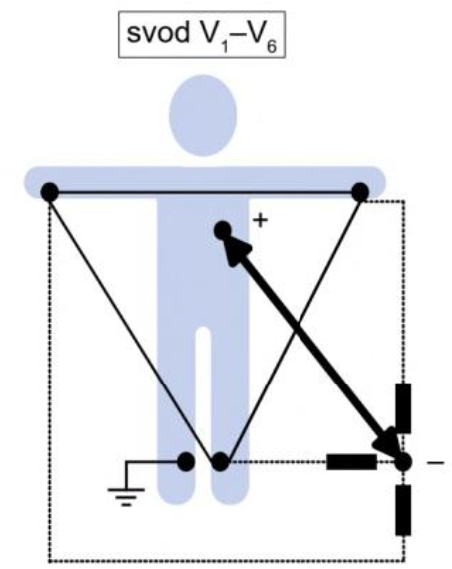
\includegraphics[height=5cm]{../assets/anatomy/unipolar2}}
		      \hfill
		      \subcaptionbox{Přiložení unipolárních hrudních svodů podle Wilsona
			      (vlevo) a přiřazení elektrod k srdci v příčném průřezu (vpravo)
			      \cite{Haberl2012}}
		      [.6\linewidth]{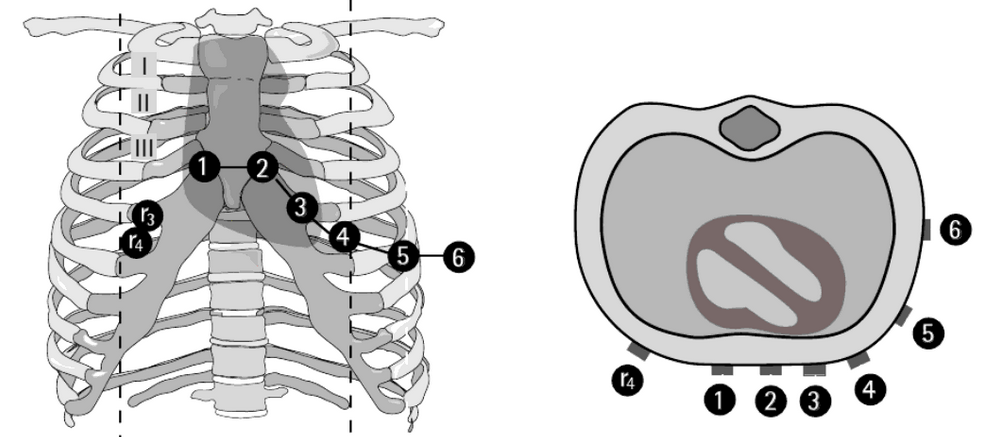
\includegraphics[height=4cm]{../assets/anatomy/unipolar3}}
		      \caption{Wilsonovy unipolární hrudní svody}
		      \label{fig:wilson}
	      \end{figure}
\end{enumerate}

Kombinací všech výše zmíněných svodů vzniká standardní klinický 12-svodový EKG
záznam, který se běžně používá v praxi. Někdy se využívají i další přídatné
svody, jako například etážové, ortogonální nebo jícnové svody. Graficky se
zaznamenává na milimetrový papír nebo je vidět na obrazovce v digitalizované
podobě. Délka záznamu se obvykle liší v závislosti na prováděné diagnostice či
terapii. K záznamu se používají různé typy EKG přístrojů, které často snímají
více biologických veličin, něž pouze elektrickou aktivitu srdce. Mezi přístroje,
které se k měření využívají, se řadí například pacientské monitory vitálních
funkcí nebo v případě mobilnějšího řešení Holterův monitor (Holter). Holterovo
monitorování se nejčastěji uplatňuje u dlouhodobého kontinuálního záznamu
srdeční aktivity, obvykle 24 hodin, kde je třeba v rámci diagnostiky sledovat
příležitostné srdeční úkazy. Největší výhodou v případě Holtru je jeho malá
konstrukce v podobě krabičky o velikosti většího mobilního telefonu což umožňuje
jeho jednoduchou přenosnost \cite{Surawicz2008}.

%//TODO: Rewrite and cite this subsection 9, 10
\subsection{Zpracování záznamu srdeční aktivity}
\label{section:ecg_processing_theory}
Monitorování či analýza EKG tvoří nepostradatelnou část v mnoha diagnostických a
terapeutických případech. Díky mobilním implementacím, pomocí kterých lze
sledovat tuto biologickou aktivitu skrze chytrá zařízení je to v současnosti
trend. Než se ale na výstupu, například v podobě displeje, objeví EKG křivka či
jiné vypočtené parametry, tak se signál musí předzpracovat, jinak by tyto
parametry byly v praxi zavádějící.

Biologické signály se zpravidla předzpracovávají použitím filtrů. Filtrace
signálu mění tvar a spektrum původního sígnálu, čímž dochází ke zvýraznění nebo
potlačení specifických složkek signálu. V případě EKG signálu se jedná o složky
v jeho frekvenční doméně, reprezentované harmonickými komponenty, které popisují
relace mezi amplitudou a časem. Tyto vztahy se mění filtrací \cite{Jan2002}. Na
základě původu a povahy signálu se filtry dělí na analogové, diskrétní a
číslicové (digitální). Navzájem se mezi sebou liší způsobem provedení náležitých
operací \cite{Skop1994}. Analogové filtry jsou realizovány v podobě RLC článků,
které se skládají z rezistorů (R), cívek (L) a kondenzátorů (C). Dále se články
dělí na pasivní a aktivní, které využívají zesilovače. Diskrétní a digitální
filtry představují spíše algoritmy než obvody \cite{Prchal2000}. Jelikož je v
této práci především použita lineární digitální filtrace, bude nadále detailněji
rozebrána oblast diskrétních lineárních časově invariantních systémů (DLI), a to
konkrétně lineární časově invariantní filtry \cite{Jan2002}.

Před samotnou filtrací se obvykle provádí spektrální analýza signálu neboli
převod signálu z časové domény do frekvenční pomocí Fourierovy transformace
(FFT), což poskytuje informace o jeho frekvenčním složení \cite{Prchal2000}.
Díky získané frekvenční charakteristice a znalosti užitečného frekvenčního
rozsahu komponentů EKG signálu a šumu je navržen filtr, který má za úkol
potlačit vliv nežádoucích interferencí.

\begin{figure}[h]
	\begin{center}
		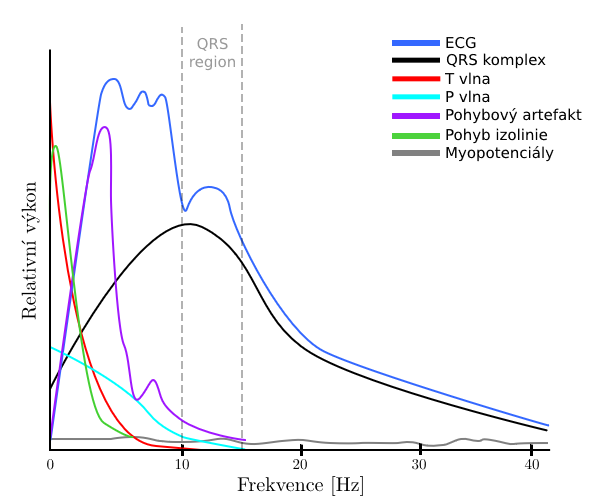
\includegraphics[width=0.7\textwidth]{../assets/figures/ecg_spectrum}
		\caption{Spektrum EKG komponentů a artefaktů [zdroj: autor]}
		\label{fig:ecg_spectrum}
	\end{center}
\end{figure}

Digitální filtry se navrhují tak, aby jejich vlastnosti splňovaly nároky, které
jsou obvykle kladeny ve kmitočtové oblasti. Mezi tyto vlastnosti se primárně
řadí amplitudová a fázová charakteristika. Realizace filtru následně probíhá
určením a optimalizací vypočítaných koeficientů společně s jejich počtem tak,
aby se frekvenční charakteristika navrženého filtru co nejvíce přibližovala
požadované frekvenční charakteristice, specifikované realizovatelnou DLI
strukturou. Podle frekvenční charakteristiky se rozlišují 4 základní typy
filtru: dolní propust (DP, lowpass filter), horní propust (HP, highpass filter),
pásmová propust (PP, bandpass filter) a pásmová zádrž (PZ, notch filter). Na
Obr. \ref{fig:amp_characteristics} jsou ideální amplitudové charakteristiky
nerealizovatelných DLI struktur ($|H_i(\widetilde\omega)|$), kterých se reálné
realizace zmíněných základních filtrů snaží dosáhnout
\cite{Skop1994,Prchal2000}. V praxi se počítá s jistou tolerancí, která
vyjadřuje kolísání od ideální amplitudové charakteristiky. K zobrazení tolerancí
filtru se používají toleranční diagramy \cite{Prchal2000,Lyons1997}.

\begin{figure}[h]
	\centering
	\begin{minipage}[b]{0.4\textwidth}
		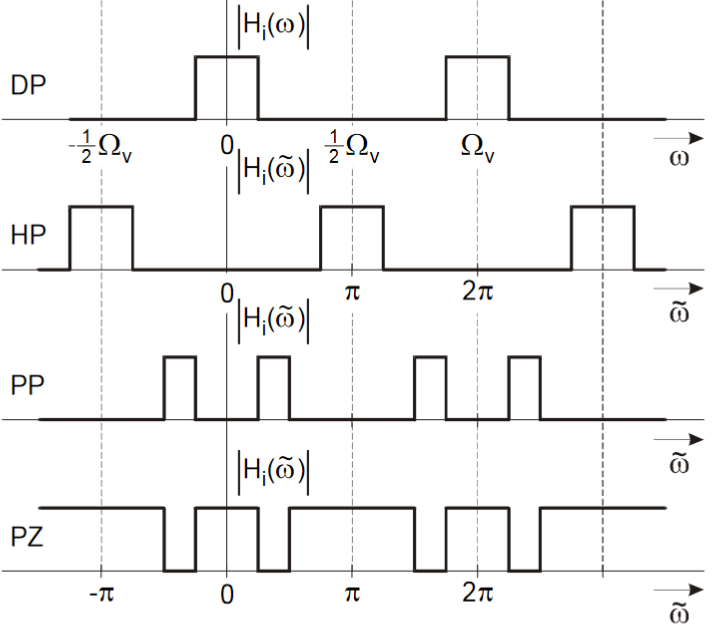
\includegraphics[width=1\linewidth]{../assets/figures/amp_characteristics}
		\caption{Ideální amplitudové charakteristiky \cite{Skop1994}}
		\label{fig:amp_characteristics}
	\end{minipage}
	\hfill
	\begin{minipage}[b]{0.5\textwidth}
		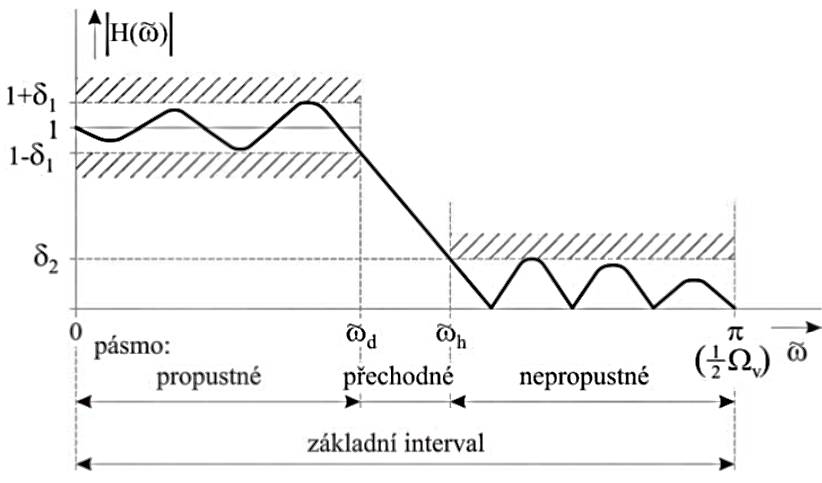
\includegraphics[width=1\linewidth]{../assets/figures/tolerance_diagram}
		\caption{Toleranční diagram filtru typu DP \cite{Skop1994}}
		\label{fig:tolerance_diagram}
	\end{minipage}
\end{figure}

V tolerančním diagramu na Obr. \ref{fig:tolerance_diagram} jsou znázorněny
další parametry, na které je také třeba dbát při návrhu filtru. Oscilacím,
viditelným v propustném a nepropustném pásmu, se přezdívá vlněni. Parametr
\textdelta \textsubscript{1} (passband ripple), vyjadřuje variaci amplitudy v
propustném pásmu navrženého filtru a je roven maximální odchylce o jednotkové
velikosti. Parametr \textdelta \textsubscript{2} (stopband attenuation) je
velikost odezvy útlumu, která vyjadřuje maximální ztrátu signálu v nepropustném
pásmu a rovná se maximální odchylce od 0. Frekvence \textomega \textsubscript{d}
a \textomega \textsubscript{h} určují šířku přechodného pásma
\cite{Prchal2000,Lyons1997}. Přechodové pásmo, zejména jeho sklon, se odvíjí od
složitosti filtru a je jedním z hlavních východisek při posuzování kvality
navrženého filtru \cite{Jan2002}.

Další důležitou vlastností, ze které se vychází při návrhu digitálních filtrů,
je impulzní odezva. Tato vlastnost dělí digitální filtry na filtry s konečnou
impulzní odezvou (FIR) a nekonečnou impulzní odezvou (IIR) \cite{Skop1994}.

Použití filtrů s konečnou impulzní odezvou má výhodné uplatnění především tehdy,
když je potřeba lineární fázové charakteristiky. Lineární fáze způsobuje
ekvivalentní fázovy posun všech frekvencí v čase, tudíž je zachované stejné
zpoždění signálu na výstupu ve srovnání se vstupním signálem. FIR filtry se dají
navrhnout s přesně lineární fázovou charakteristikou, pokud je jejich impulzní
odezva symetrická nebo asymetrická \cite{Prchal2000}. Matematická definice
filtru vychází z principu superpozice DLI systémů a je definována jako konečná
diskrétní konvoluce \cite{Jan2002}:

\begin{equation}
	\label{eq:conv_fir}
	y_n = \sum_{k=1}^{N-1} k_{n-k} h_k
\end{equation}

kde $N$ je řád filtru, $x$ vstupní signál a $h$ je vektor obsahující koeficienty
impulzní odezvy filtru pro které platí $n \in \langle 0,N-1 \rangle$
\cite{Jan2002}. Stabilita filtrů vychází ze z-transformace impulzní odezvy:

\begin{equation}
	\label{eq:transfer_fir}
	H(z) = \sum_{n=0}^{N-1} h_n z_{-n}
\end{equation}

která je po transformaci ve své rovině dána jen nulovými body \cite{Jan2002}.
Frekvenční charakteristika filtrů:

\begin{equation}
	\label{eq:freq_fir}
	G(\omega) = H(e^{j \omega T}) = \sum_{n=0}^{N-1} h_n e^{-j \omega T}
\end{equation}

je spojitá periodická funkce s periodou $2\pi/T$ \cite{Jan2002}. Jelikož je
frekvenční charakteristika $G(\widetilde\omega)$ spojená s impulzní odezvou
$h(n)$ Fourierovou transformací \cite{Prchal2000}, tak koeficienty impulzní
odezvy $h_n$ vycházejí z Fourierovy řady. Díky tomu lze filtry tohoto typu
poměrně snadno navrhnout \cite{Jan2002}. Další vlastnosti FIR filtrů, které
mohou sloužit jako rozhodovací kritérium při návrhu filtru jsou
\cite{Prchal2000}:

\begin{itemize}
	\item Absolutní stabilita,
	\item Nerekurzivní struktura,
	\item Jednoduchá implementace,
	\item Vysoká výpočetní náročnost.
\end{itemize}

Pokud lineární fázová charakteristika nehraje roli, volí se spíše filtry typu
IIR. Filtry tohoto typu umožňují dosáhnout stejné útlumové charakteristiky jako
u FIR filtrů při menším počtu koeficientů \cite{Prchal2000}. Výhoda malé
výpočetní náročnosti IIR filtrů má uplatnění primárně ve zpracování signálu v
reálném čase. Další velkou výhodou je široký rozsah realizací, hlavně možnost
návrhu IIR filtru s podobnými charakteristikami analogových filtrů
\cite{Jan2002,Lyons1997}. Populární biomedicínské IIR implementace analogových
filtrů jsou především Butterworthovy, Čebyševovy (Chebyshev), Besselovy a
Eliptické filtry \cite{Paarmann2006}. Návrh IIR filtrů je komplikovanější než u
FIR filtrů a často může představovat složitou optimalizační úlohu. Matematicky
jsou IIR filtry definované rekurzivními diferenčními rovnicemi: \cite{Jan2002}:

\begin{equation}
	\label{eq:conv_iir}
	y_n = \sum_{i=0}^{r} L_i x_{n-1} - \sum_{i=1}^{m} K_i y_{n-1}
\end{equation}

kde $r$ spolu s $L_i$ je řád a koeficienty nerekurzivní části filtru. Naopak $m$
je řád a $K_i$ jsou koeficienty rekurzivní části filtru. Obecně platí $r \leq m$
\cite{Jan2002,Prchal2000}. Přenosová funkce:

\begin{equation}
	\label{eq:transfer_iir}
	H(z) = \frac{\sum_{i=0}^{r} L_i z^{m-i}}{\sum_{i=0}^{m} K_i z^{m-i}} = A \frac{\prod_{i=1}^{r} (z-n_i)}{\prod_{i=1}^{m} (z-p_i)}
\end{equation}

je v z-rovině vyjádřená podílem polynomů, kde $Li$ $Ki$ jsou systémové
konstanty. Často se lze setkat s následným součinovým vyjádřením, které filtr
popisuje pomocí konfigurace pólů $p_i$, nulových bodů $n_i$ a zesílení $A$
\cite{Jan2002,Prchal2000}. Vyjádření frekvenční charakteristiky je v případě IIR
filtrů složitější a obvykle se používa k popisu spíše vztah pro amplitudovou a
fázovou charakteristiku:

\begin{equation}
	\label{eq:ampphase_iir}
	|G(\omega)| = A \frac{\prod_{i=1}^{r} d_i}{\prod_{i=1}^{m} l_i} ~a~ arg(G(\omega)) = (m-r)\omega T + \sum_{i=1}^{r} \Phi_i - \sum_{i=1}^{m} \Psi_i
\end{equation}

kde $d_i$ spolu s $l_i$ jsou vzdálenosti mezi bodem $e^{j\omega T}$ a nulami
(póly). $\Phi_i$ a $\Psi_i$ jsou úhly náležitých spojnic
\cite{Prchal2000,Jan2002}. Níže jsou další vybrané vlastnosti IIR filtrů
\cite{Jan2002}:

\begin{itemize}
	\item Rekurzivní struktura,
	\item Nízka latence zpracování,
	\item Nelineární fázová charakteristika,
	\item Menší stabilita.
\end{itemize}

\begin{figure}[h]
	\begin{center}
		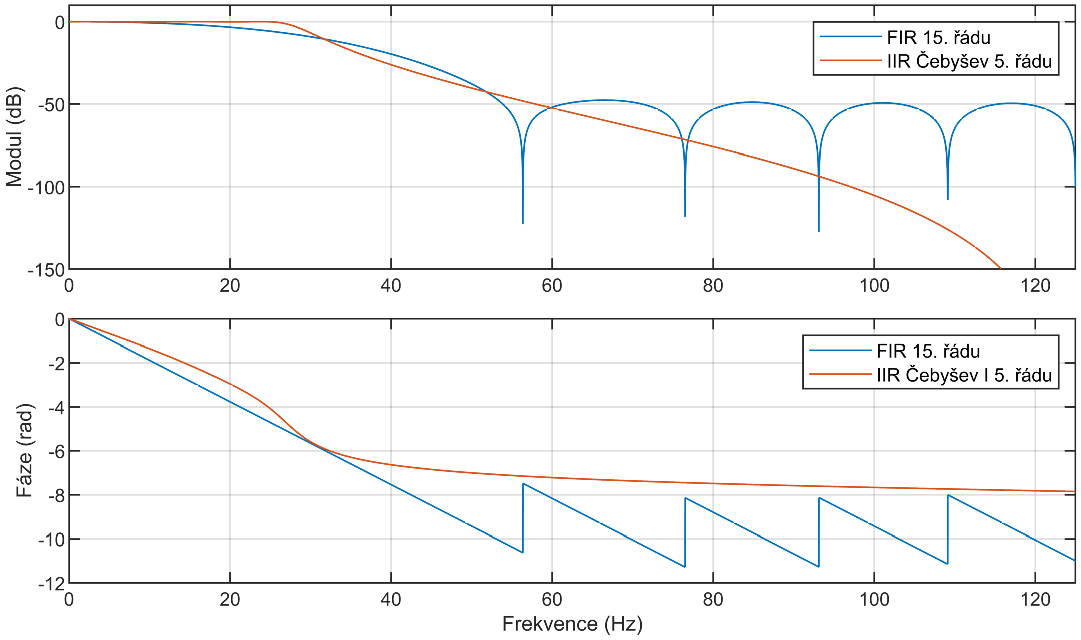
\includegraphics[width=1\textwidth]{../assets/figures/filters_comparison}
		\caption{Rozdíl amplitudové a fázové frekvenční charakteristiky FIR a IIR filtru [zdroj: autor]}
		\label{fig:filters_comparison}
	\end{center}
\end{figure}

Rozdíl mezi FIR a IIR filtry je viditelný vzájemným porovnáním jejich impulsní a
frekvenční charakteristiky. Na Obr. \ref{fig:filters_comparison} jsou graficky
znázorněny tyto charakteristiky pro FIR filtr 15. řádu a Čebyševův filtr 5. řádu
typu I. Filtry byly navrženy jako dolní propust s mezní frekvencí 25 \si\Hz. I
přes značný grafický rozdíl impulsních charakteristik je útlumová úroveň filtrů
velmi podobná, avšak výpočetně IIR filtru stačilo 6 koeficientů oproti FIR
filtru, který jich vyžadoval 15. Hlavní rozdíl vyplívá především z fázové
charakteristiky, kde se v propustném pásmu, a hlavně kolem mezní frekvence
projevuje nelineární fázový charakter IIR filtru.

Včetně lineárních metod filtrace se v praxi často užívají i další metody
předzpracování mezi které se řadí například nelineární a adaptivní filtrace
\cite{Sornmo1982,Pan1985}, vlnkové transformace \cite{Yao2020,Ndiaye2020},
korelační analýza, kumulační metody nebo se využívá neuronových
sítí\cite{Kiranyaz2016,Zhai2018} \cite{Jan2002}. Po filtraci signálu a potlačení
nežádoucích rušivých složek přichází na řadu jeho segmentace a extrakce
komponentů potřebných k analýze. Na extrahované komponenty se následně aplikují
další postupy hodnotící fyziologické jevy, mezi které nejčastěji patří HRV.

\subsubsection{Nežádoucí elementy EKG signálu}
EKG signál často zkreslují mnohočetné okolní a elektrofyziologické vlivy, které
mohou vést k jeho nesprávné interpretaci. Nejčastější rušivé prvky, které se
projevují na signálu jsou: síťový brum, myopotenciály, pohybové artefakty nebo
špatné umístění elektrod. \cite{Surawicz2008}.

Sítový brum neboli elektrická interference generovaná střídavým proudem ze
zásuvky, je jedním z nejběžnějších artefaktů projevujících se u biologických
signálu. Příčinou jeho vzniku může být špatné uzemnění či chod zařízení nebo
vliv elektromagnetického rušení okolní techniky v blízkosti měřícího přístroje.
Na Obr. \ref{fig:ac_Interference} je vidět vliv střídavého proudu o frekvenci 50
\si\Hz~na EKG signál \cite{Goldberger2017}. Nejčastěji se k eliminaci
úzkopásmového rušení tohoto typu volí filtry navržené jako pásmová zádrž, které
nepropouští specifikované frekvence signálu \cite{Kher2019}.

\begin{figure}[h]
	\begin{subfigure}[b]{0.5\linewidth}
		\centering
		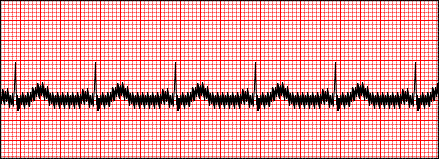
\includegraphics[width=0.8\linewidth]{../assets/ecg/ac_Interference}
		\caption{AC rušení}
		\label{fig:ac_Interference}
		\vspace{4ex}
	\end{subfigure}
	\begin{subfigure}[b]{0.5\linewidth}
		\centering
		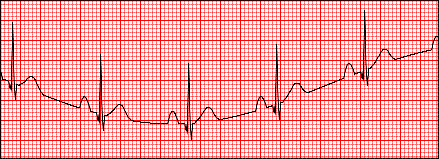
\includegraphics[width=0.8\linewidth]{../assets/ecg/w_baseline}
		\caption{Pohyb izoelektrické linie}
		\label{fig:w_baseline}
		\vspace{4ex}
	\end{subfigure}
	\begin{subfigure}[b]{0.5\linewidth}
		\centering
		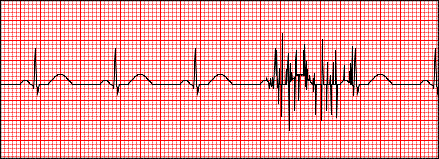
\includegraphics[width=0.8\linewidth]{../assets/ecg/muscle_tremor}
		\caption{Myopotenciály (svalový třes, tremor)}
		\label{fig:muscle_tremor}
	\end{subfigure}
	\begin{subfigure}[b]{0.5\linewidth}
		\centering
		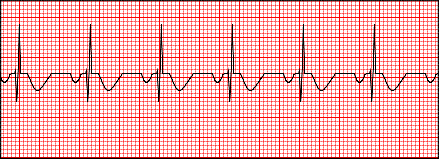
\includegraphics[width=0.8\linewidth]{../assets/ecg/rev_electrodes}
		\caption{Nesprávné umístění elektrod}
		\label{fig:rev_electrodes}
	\end{subfigure}
	\caption{Běžné EKG artefakty \cite{Mauvila2004}}
	\label{fig:common_artifacts}
\end{figure}

Pohybové artefakty se primárně na EKG signálu projevují kolísáním elektrické
izolinie (drift) od její nulové hodnoty jako je tomu na Obr.
\ref{fig:w_baseline}. Nevznikají však pouze pohybem pacienta ale i například
manipulací měřicími kabely, špatným kontaktem elektrod nebo vlivem dýchání
pacienta \cite{Goldberger2017}. V lepších případech stačí ke korekci driftu
filtry typu horní propusti, avšak někdy je potřeba využít například vlnkových
transformací nebo adaptivní filtrace, obzvláště v situacích fyzického pohybu
nebo špatného kontaktu elektrod \cite{Kher2019}.

Svalové artefakty neboli myopotenciály jsou dalším častým typem rušení
vysokofrekvenčního charakteru, které ovlivňuje EKG signál. Svým způsobem patří
tento typ rušení z části mezi předešlé pohybové artefakty, jelikož mohou vznikat
pohybem pacienta. Tento pohyb může být nedobrovolný například u osob trpících
Parkinsonovou chorobou, kterou obvykle doprovází svalový třes (tremor) nebo
pulzace arteriální tepny pod elektrodou \cite{Surawicz2008}. Vlivem pohybů
kosterního svalstva vzniká svalová elektrická aktivita (EMG), která náhodně
interferuje s EKG signálem. Na Obr. \ref{fig:muscle_tremor} je vidět tato
interference v podobě překrytí QRS komplexu myopotenciálem
\cite{Goldberger2017}. K potlačení myopotenciálu se často využivájí vyhlazovací
filtry nebo například filtry typu dolní propust s Gaussovou impulsní odezvou
\cite{Kher2019}. Populárním vyhlazovacím digitálním filtrem je Savitzky–Golay
filtr \cite{Schafer2011}.

V neposlední řadě, spíše než rušení, je častou chybou při záznamu EKG špatné
umístění nebo prohození elektrod. Proto je nutné pamatovat si význam barev
elektrod. Každá barva označuje specifické místo na těle, kam má být elektroda
připevněna. Pokud dojde k prohození, dochází k měření jiného chybného
potenciálu. Na Obr. \ref{fig:rev_electrodes} je vidět situace, kdy došlo k
záměně bíle a červené elektrody. Výsledkem je inverze všech vln EKG křivky (P,
Q, R, S, T) \cite{Goldberger2017,Surawicz2008}.

\subsubsection{Detekce EKG komponentů}
\label{section:components_detection_theory}
Detekce, segmentace a extrakce EKG komponentů, nejčastěji QRS komplexu, je v
posledním století velmí žhavé téma, které těží z rozvoje výpočetní techniky.
Největší zlom nastal při vzniku neuronovýh sítí a příchodu umělé inteligence,
která přinesla v této oblasti nespočet nových řešení, primárně v automatizované
detekci a klasifikaci kardiovaskulárních onemocnění \cite{Kashou2020}. I
přestože softwarové implementace detektorů čim dál častějí nahrazují hardwarová
řešení, tak po hardwarové stránce dochází v rozvojí hlavně v mobilních
zařízeních \cite{Kohler2002}.

\begin{figure}[h]
	\centering
	\begin{tikzpicture}[node distance=2.5cm, thick, scale=0.85, every node/.style={scale=0.9}]
		\node (pro1) [process, xshift=2cm, text width=2cm] {Lineární filtrace};
		\node (pro2) [process, right of=pro1, xshift=0.8cm, text width=2cm] {Nelineární filtrace};
		\node (Title1) [text=black!50, below of=pro1, node distance=1.2cm, xshift=1.7cm] {Předzpracování};
		\node (blok1) [draw=black!50, dashed, inner sep=0.4cm, fit={(pro1) (pro2) (Title1)}] {};
		\node (start) [left of=blok1, node distance=5cm] {};

		\node (pro3) [process, right of=pro2, xshift=2cm, text width=2cm] {Detekční algoritmus};
		\node (pro4) [process, right of=pro3, xshift=0.8cm, text width=2cm] {Rozhodovací pravidlo};
		\node (Title2) [text=black!50, below of=pro3, node distance=1.2cm, xshift=1.7cm] {Rozhodování};
		\node (blok2) [draw=black!50, dashed, inner sep=0.4cm, fit={(pro3) (pro4) (Title2)}] {};
		\node (stop) [right of=blok2, xshift=1.5cm] {};

		\draw [arrow] (start) -- node [above] {EKG} (blok1);
		\draw [arrow] (blok1) -- (blok2);
		\draw [arrow] (blok2) -- (stop);
	\end{tikzpicture}
	\caption{Běžná struktura QRS detektorů \cite{Kohler2002}}
	\label{fig:qrs_detection}
\end{figure}

Prvním východiskem detekce je oblast analýzy, od které se odvíjí potřebné
komponenty a jejich doména. Oblast může být časová nebo frekvenční. Dalším
krokem je výběr nebo návrh samotné metody pro detekci. Nejčastějším případem v
rámci EKG signálu je detekce QRS komplexu, případně jeho dílčích částí. EKG
signál se následně segmentuje na jednotlivé úseky v závislosti na detekovaných
komplexech \cite{Canento2012}. Detekční algoritmy zpravidla obsahují další
filtry a matematické operace zvýrazňující QRS komplexy spolu s rozhodovacími
pravidly. Rozhodovací pravidla si lze představit jako podmínky, jejichž splněním
je definován nalezený komponent. Z hlediska principu předzpracování se často
používají například algoritmy založené na \cite{Kohler2002,Vaneghi2012}:

\begin{itemize}
	\item \textit{digitální filtraci} \cite{Sornmo1982,Kesel1997481},
	\item \textit{diferenciaci} \cite{Tompkins1983,Okada1979},
	\item \textit{vlnkové transformaci} \cite{Yao2020,Ndiaye2020},
	\item \textit{počítání průchodů nulou} \cite{Kohler2003,Turnip2018},
	\item \textit{Hilbertově transformaci} \cite{Valluraiah2015, Ouali2020},
	\item \textit{matematické morfologii} \cite{Li1999,Tadejko2007},
	\item \textit{použití neuronových sítí} \cite{Kiranyaz2016,Zhai2018}.
\end{itemize}

Většina nově vzniklých metod často čerpá a kombinuje poznatky z těch, které se
postupem času staly konvenčními. Nejznámějším případem takové metody, kterou lze
nazývat konvenční, je Pan-Tompkinsův algoritmus \cite{Pan1985}.

QRS detekční aloritmus, který navrhl a realizoval Pan-Tompkins v roce 1985, je
doposud jedním z nejpopulárnějších algoritmů v oblasti zpracování EKG signálu.
Navržen byl primárně pro aplikace v reálném čase. Algortimus má dvě hlavní
části, předzpracování signálu a rozhodovací část. Část předzpracování používá 3
typy filtrů --- pásmová propust, derivační filtr, integrační filtr --- k
potlační šumu a artefaktů signálu \cite{Alvarez2013}. Derivační filtr potlačuje
vlivy P a T vln. Integrační filtr, se aplikuje v podobě pohyblivého okna pro
vyhlazení signálu \cite{Pan1985}. Rozhodovací část neboli část zpracování, se
věnuje detekci QRS komplexů. Pro zvýšení spolehlivosti algoritmu probíha detekce
zároveň na derivovaném a na vyhlazeném signálu. Prvotním krokem je nalezení
lokálních maxim v podobě R vln. Následně se aplikuje adaptivní prahování formou
pohyblivého okna pří kterém jsou rozhodovacím pravidlem vybrány pouze R vlny
překračující prahovou hodnotu. Vybrané R vlny představují referenční body
detekovaných QRS komplexů \cite{Pan1985,Alvarez2013}.

\begin{figure}[H]
	\centering
	\begin{tikzpicture}[node distance=2.5cm, thick, scale=0.85, every node/.style={scale=0.85}]
		\node (start) [startstop] {Vstupní EKG signál};
		\node (pro1) [process, below of=start, yshift=1cm] {Pásmová propust};
		\node (pro2) [process, right of=pro1, xshift=2cm] {Derivační filtr};
		\node (pro3) [process, right of=pro2, xshift=2cm] {Umocnění signálu};
		\node (pro4) [process, right of=pro3, xshift=2cm] {Integrační filtr};
		\node (pro5) [process, below of=pro4, text width=3cm] {Počáteční detekce R vln};
		\node (pro6) [process, below of=pro3, text width=3cm] {Adaptivní prahování};
		\node (pro7) [process, below of=pro2, text width=3cm] {Rozhodovací pravidlo};
		\node (stop) [startstop, below of=pro1] {QRS komplex};

		\draw [arrow] (start) -- (pro1);
		\draw [arrow] (pro1) -- (pro2);
		\draw [arrow] (pro2) -- (pro3);
		\draw [arrow] (pro3) -- (pro4);
		\draw [arrow] (pro4) -- (pro5);
		\draw [arrow] (pro5) -- (pro6);
		\draw [arrow] (pro6) -- (pro7);
		\draw [arrow] (pro7) -- (stop);
	\end{tikzpicture}
	\caption{Pan-Tompkinsův algoritmus [zdroj: autor]}
	\label{fig:pan_tompkins}
\end{figure}

Existuje mnoho dalších QRS detektorů, jejichž řešení se orientuje především
povahou dat a způsobem zpracování. Způsobem zpracování se rozumí, zdali detekce
probíhá na již naměřených datech --- offline --- nebo v reálném čase --- online.
Povaha dat je dána způsobem měření. Záznamy srdeční aktivity naměřené
intrakardiálně nejsou zatížené artefakty tolik jako záznamy pořízené
Holterovským monitorováním. Z toho vyplivá i komplexita detektoru, jelikož EKG
záznamy zatížené mnohočetnými artefakty vyžadují mnohem sofistikovanější
detekční algoritmy. Další populární QRS detektory a jejich srovnání je rozebráno
v \cite{Kohler2002,Canento2012,Vaneghi2012,Alvarez2013,Karpagachelvi2010}.


%//TODO: Rewrite and cite this subsection 9, 10
\subsection{Variabilita srdeční frekvence}
\label{section:hrv}
Jednou z nejčastěji sledovaných elektrofyziologických veličin je srdeční rytmus.
Je to veličina, měnící se s každým dalším úderem srdce, ovlivňována aktivitou
ANS. Jelikož srdeční rytmus vychází normálně ze sinoatriálního uzlu, jedná se o
sinusový rytmus závislý na tonu sympatiku a parasympatiku. Proto se mezi
faktory ovlivňující srdeční rytmus řadí vnější a vnitřní vlivy jako vznik
ischemie, metabolická dysbalance nebo zvýšená kognitivní, emoční a fyzická
zátěž, které jsou zároveň stěžejními pro rozbor samotného EKG záznamu
\cite{Pumprla2014}. Blíže jsou tyto vztahy popsány v sekci
\ref{section:hr_regulation}. Autonomní procesy regulující srdeční činnost nebo
jiné aktivity podmíněné fyziologickými a psychofyziologickými vlivy se včetně
změny rychlosti srdečního rytmu promítají jako časové variace mezi jednotlivými
stahy srdce. Časové variace neboli lišící se délky jednotlivých R-R intervalů se
obecně označují jako variabilita srdečního rytmu.
\cite{Pumprla2014,Rajendra2007}.

Z HRV vycházejí i další parametry, které se využívají k jejímu hodnocení.
Výpočet a smysl specifických parametrů už spadá pod jednotlivé metody hodnocení
HRV v následující kapitole. K tomu aby bylo možné HRV kvantitativně hodnotit je
potřeba z EKG signálu extrahovat R vlny, jejichž časová diference je právě
hledanou variabilitou. Artefakty EKG mohou v případě HRV analýzy hrát stěžejní
roli pokud došlo k zániku nebo významnému zkreslení některých R vln. Nejčastěji
se u zaniklých R vln používají metody lineární interpolace, které zachovávají
správnou variabilitu. Srovnání rozdílných metod interpolace, včetně té lineární
a dopad chybějících R vln na HRV analýzu již bylo popsáno v
\cite{Kim2007,Peltola2012,Morelli2019}. Další častou příčinou abnormálních R
vln, se kterou se lze v praxi setkat, jsou ektopické stahy. Proto existuje mnoho
algoritmů, které se věnují zpracování R-R intervalů aby bylo možné HRV hodnotit
\cite{Lipponen2019}.

\subsubsection{Metody hodnocení HRV}
\label{section:hrv_methods}
Hodnocení variability srdečního rytmu neboli zkoumání variace mezi jednotlivými
srdečními stahy nachází dnes velké uplatnění v diagnostice, například v rámci
rychlého neinvazivního zhodnocení kardiovaskulární autonomní regulace.
Nejčastější a základní neinvazivní metody hodnocení HRV mohou být sjednoceny do
časové a frekvenční oblasti ale existují i další geomterické a nelineární
postupy. Nejzákladnější běžná metoda je spektrální analýza variability srdečního
rytmu, která umožňuje zaznamenat a deklarovat vlivy kardiálního autonomního
nervového systému \cite{Pumprla2014}. Často se lze setkat, primárně u hodnocení
dlouhodobých EKG záznamů, se statistickou analýzou, která využívá parametry
vypočítané z HRV v časové doméně. Hodnoty jednotlivých parametrů následně slouží
jako indikátory změn pro různé oblasti kardiovaskulárního systému a ANS
\cite{Malik1996}. Časové a frekvenční metody mají však své technické omezení
jako například předpoklad linearity dat a v některých případech se neumějí
vypořádat s interferencemi způsobené ektopickým rytmem \cite{Hsu2012}. Další
populární geometrickou nelineární metodou je analýza Poincarého grafu, na kterém
je každý R-R interval vynesen proti nadcházejícímu R-R intervalu. 

Poincarého graf (plot) lze interpretovat jako kartezský souřadnicový systém
tvořící mapu bodů, kde každý bod je definován dvojící $RR_i$ (osa x) a
$RR_{i+1}$ (osa y) \cite{Hsu2012,Hejjel2001}. Narozdíl od předešlých metod se
Poincarého graf vyhodnocuje jak kvalitativně, pomocí tvaru (vzoru) vzniklého z
bodů, tak i kvantitativně, výpočtem SD indexů grafu, které poskytují podobné
informace jako LF a HF složky spektrálního výkonu nebo statistické parametry
SDNN a RMSSD. Z grafu tak lze získat souhrné i detailní informace o dynamickém
chování srdečního rytmu \cite{Hsu2012,Kubickova2016}. 

\begin{figure}[h]
	\begin{center}
		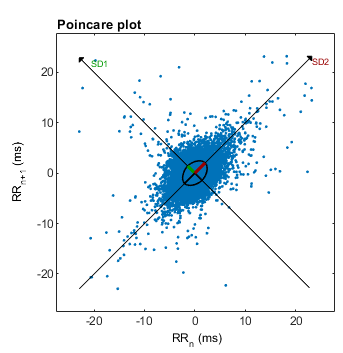
\includegraphics[width=0.5\textwidth]{../assets/figures/wiki_poincare}
		\caption{Poincarého graf \cite{wikiPoincare}}
		\label{fig:wiki_poincare}
	\end{center}
\end{figure}

Jak již bylo zmíněno, kvalitativní analýza se orientuje rozložením bodů na
Poincarého grafu a vypovídá o variabilitě. Čím menší je plocha vzoru bodů, tím
menší je variabilita, a naopak. Disperze bodů podél osy grafu procházející
počátkem vypovídá a dlouhodobě variabilitě a rozptýlení bodu kolmo na tuto osu o
krátkodobé. Průnikem diagonálních os grafu je průměrná hodnota R-R intervalů
\cite{Hejjel2001}. Poloha shluku bodů na diagonále procházející počátkem hraje
také roli. Pozice shluku blíže počátku indikuje vliv sympatiku zatímco pozice
dál směrem na opačnou stranu vliv parasympatiku. Pokud se v grafu nachází více
shluků lze očekávat arytmie. Asymetrie vzoru bodů může vypovídat o poruchách
srdečního rytmu \cite{Habib2013}. Vizuální charakteristiky Poincarého grafu se
dají vyjádřit i kvantitativně. Nejpopulárnější technikou kvantitativního
hodnocení Poincarého grafu je konstrukce elipsy podle vzoru bodů. Z hlavní a
vedlejší osy elipsy lze vypočítat indexy SD1 a SD2. Tvarové vlasnosti elipsy
jsou v souladu se zmíněnými vlasnosti tvaru shluku bodů výše. SD indexy jsou
směrodátné odchylky okamžité variability ve směru osy
\cite{Habib2013,Mazhar2007}.

Všechny metody jsou pak v praxi využitelné pro včasné odhalení
kardiovaskulárních onemocnění, nicméně jsou použitelné pouze ve specifických
laboratorních podmínkách a jako jiné jsou ovlivnitelné právě fyzickými a
psychologickými faktory \cite{Habib2013,Kubickova2016}. Parametry HRV můžou
sloužit pro predikci kognitivní zátěže, ale pro jejich spolehlivé určení je
nezbytný pečlivý výběr vhodných metod předzpracování signálu.

\subsubsection{Model neuroviscerální integrace}
Model neuroviscerální integrace popisuje vztahy v rámci periferní
psychofyziologie, neurověd a autonomních funkci spjatých s regulací vagálního
tonu. Tyto znalosti a vztahy jsou kombinovány do několika detailně popsaných
teoretických vrstev, dohromady tvořících jediný framework sloužící také jako
prediktivní model, který pak usnadňuje vyhodnotit souvislosti a důsledky
zásadních fyziologických změn srdeční aktivity či veličin s ní spojených
\cite{Smith2017}.

\begin{figure}[h]
	\begin{center}
		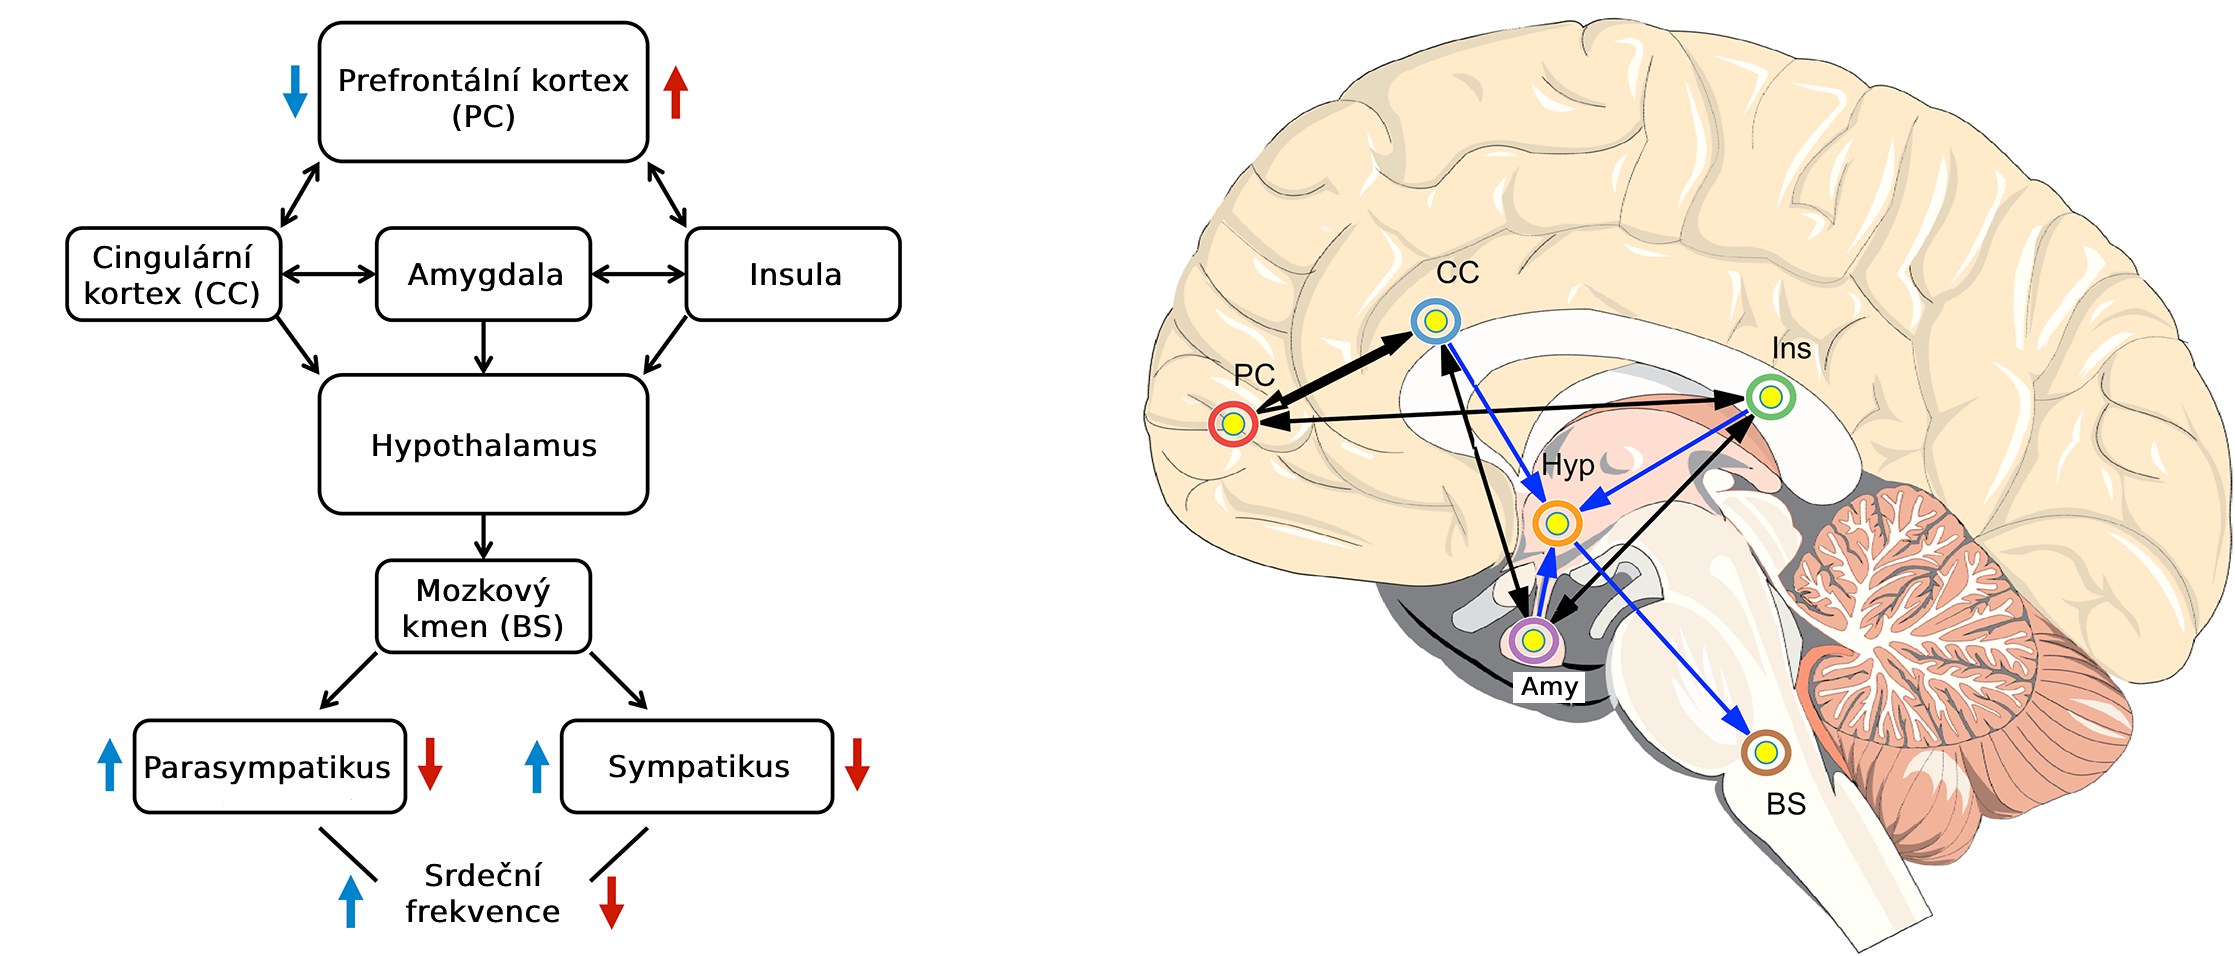
\includegraphics[width=1\textwidth]{../assets/diagrams/nvi}
		\caption{Zjednodušený model neuroviscerální integrace (Upraveno a převzato z \cite{NVI20017})}
		\label{fig:nvi_model}
	\end{center}
\end{figure}

Souvislosti modelu NVI mají například za následek, že odlišné druhy kognitivní
zátěže se promítají do časové a frekvenční domény EKG signálu. Specificky se
projevují jako kvantitativní lineární a nelineární časové parametry nebo velmi
nízko, nízko a vysoko frekvenční složky (VLF, LF, HF) výkonového spektra.
Jednotlivé komponenty slouží pří samotné analýze jako indikátory činnosti
vegetativní nervové soustavy (VNS). Aby bylo ale možné tyto komponenty získat a
porovnávat či jakkoliv hodnotit srdeční aktivitu, musí být záznam srdeční
aktivity patřičně zpracován. Model NVI je nad rámec této práce a detailněji je
rozebrán v \cite{Smith2017}.

\subsubsection{HRV v diagnostice a terapii}
Dříve panovalo obecné přesvědčení že variace v srdečním rytmu jsou patologický
úkaz a nebylo jim věnováno žádné zvláštní pozornosti. Falešná domněnka o HRV
byla poprvé vyvrácena v roce 1978, klinickou studií \cite{Wolf1978}, která
potvrzuje korelaci snížené HRV s úmrtností a arytmickými komplikacemi během
postinfarktového období. Od té doby se studie na téma nepravidelností sinusového
rytmu začaly rozvíjet a hromadit. V současnosti je HRV klinicky významnou a
velmi využívanou biometrikou napříč obory. Na Obr. \ref{fig:hrv_infarct} níže je
vidět vývoj HRV během 24h Holterovského monitorování dvou pacientů (D, S) v
postinfarktovém období, konkrétně 7. den po infarktu myokardu. U pacienta $D$
lze pozorovat nekomplikovaný postinfarktový průběh v podobě konstantního vývoje
R-R intervalů. Pacient $S$ umřel 27. den pod infarktu \cite{Malik1990}. Další
rizikové faktory korelující s HRV parametry lze najít v tabulce
\ref{tab:hrv_factors}.

\begin{figure}[h]
	\begin{center}
		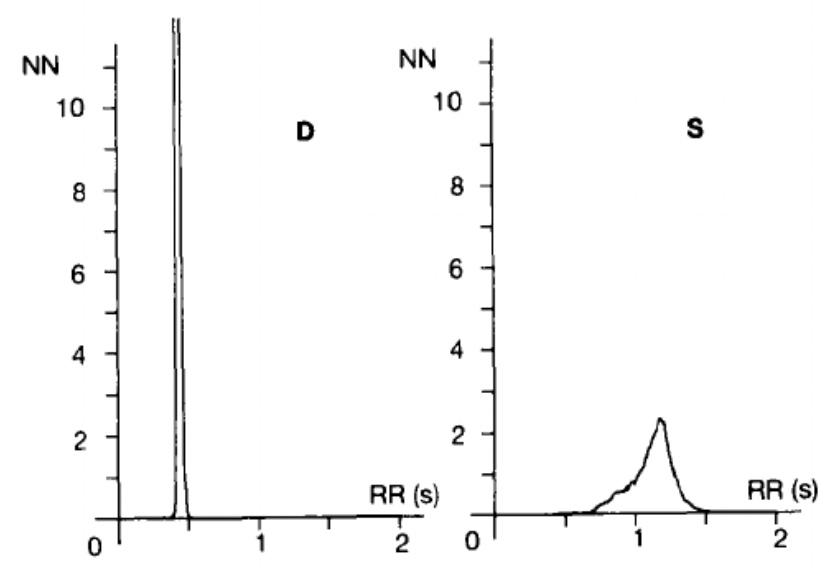
\includegraphics[width=0.5\textwidth]{../assets/figures/hrv_infarct}
		\caption{Rozdíly v HRV mezi pacienty (S, D) s vysokým a nízkým rizikem úmrtí v
			postinfarktovém období \cite{Malik1990}}
		\label{fig:hrv_infarct}
	\end{center}
\end{figure}

Ačkoli hodnocení HRV našlo pochopitelně největší praktické uplatnění v oboru
kardiologie, existují další obory, do kterých vnesla tato biometrika v
posledních letech mnoho nových poznatků. Jedním z takových oborů je psychologie
a kognitivní psychologie v rámci neuropsychofyziologických vlivů, které jsou
důsledkem změn a procesů probíhajících v ANS \cite{Bernardi2009}. Blíže je
kognitivní teorie popsána v \cite{Forte2019,Plass2010}. Studie v rámci
kognitivní psychologie
\cite{Bernardi2009,Solhjoo2019,Salahuddin2007,Ishaque2020} potvrzují, že různé
druhy kognitivní zátěže ovliňují kardiovaskulární systém, primárně HRV, a to i z
hlediska dlouhodobých korelací se statistickými HRV parametry. Proto je možné v
tabulce \ref{tab:hrv_factors} vidět faktor typu pracovního stresu, který se řadí
mezi specifický druh kognitivní zátěže.

Prognostický význám má HRV i v řadě dalších klinických a intenzivistických oborů
mezi které například patří diabetologie, renologie a neurologie. S využitím HRV
se lze dále setkat na jednotkách intenzivní péče, kde monitorování této metriky
slouží k predikci potenciálních pooperačních komplikací. Své uplatnění našla i
ve farmakokinetice při posuzování odezvy organismu na podané léčiva
\cite{Pumprla2014}.

%//TODO: Add acronyms to acronyms table ICHS, SDNN, SDNNi, RMSSD, SD1, SD2, SD1/SD2
\begin{table}[h]
	\catcode`\-=12
	\scriptsize
	\begin{center}
		\caption[HRV a rizikové faktory]{Vybrané vztahy mezi HRV parametry a rizikovými faktory
			(Upraveno a převzato z \cite{Pumprla2014,Thayer2009})}
		\label{tab:hrv_factors}
		\vspace{1ex}
		\begin{tabular}{|p{1.3cm}|p{1.7cm}|p{4.5cm}|p{5.5cm}|}
			\noalign{\hrule height 2pt}
			\textbf{Riziko} & \textbf{Autor}     & \textbf{Sledovaný parametr a populace}                                  & \textbf{Závěr}                                                                                                                                                                                  \\ \hline
			Hypertenze      & Schroeder          & HRV, hypertenze, krevní tlak. n=11061, 28\% incidence hypertenze        & 1,1–-1,6x riziko rozvoje hypertenze u subjektů s patologickými hodnotami časové analýzy HRV (SDNN, RMSSD, délka R-R int.)                                                                       \\ \hline
			Cholesterol     & Christensen        & HRV a cholesterol. n=85, 55\% s ICHS                                    & Asociace mezi nižší HRV (časová analýza, SDNN, RMSSD) a vyšším cholesterolem u pacientů s ICHS i u zdravých jedinců                                                                             \\ \hline
			Diabetes        & Liao (ARIC studie) & HRV, diabetes, glykemie, inzulinemie. n=1933, 8\% diabetiků             & Snížený výkon v HF pásmu u diabetiků ve srovnání s nediabetiky (p=0,01)                                                                                                                         \\ \hline
			Pohyb           & Sloan              & HRV, aerobní aktivita. n=149 zdravých                                   & Zvýšení SDNN a HF výkonu po 12 týdenním aerobním tréninku. Opětný pokles SDNN a HF výkonu za 4 týdny po ukončení vytrvalostního tréninku                                                        \\ \hline
			Kouření         & Hayano             & HRV, krátko a dlouhodobý efekt kouření. n=81 mužů, 69\% kuřáci          & Pokles HF výkonu již po 1 cigaretě (p=0,006). Zvýšení CCV v LF pásmu za 10–-17 min po kouření (p=0,0001). Nižší CCV v HF pásmu u těžkých kuřáků ve srovnání s nekuřáky/lehkými kuřáky (p=0,008) \\ \hline
			Pracovní stres  & van Amelsvoort     & HRV, pracovní zátěž, fyzická aktivita, pracovní směny. n=135, 84\% mužů & SDNNi během spánku: 69.3 ms proti 85.8 ms, p < 0.05, směna a denní pracovníci                                                                                                                   \\ \noalign{\hrule height 2pt}
		\end{tabular}
	\end{center}
\end{table}